\documentclass{article}
\usepackage{iclr2027_conference,times}
\usepackage{amsmath,amssymb,amsthm}
\usepackage{booktabs,multirow,graphicx,xcolor}
\usepackage{hyperref}
\usepackage{url}
\hypersetup{colorlinks=true,linkcolor=black,citecolor=black,urlcolor=black}

% Placeholder macro (no placeholders remain in this version).
\newcommand{\tbd}[1]{\textcolor{red}{[#1]}}

\newtheorem{hypothesis}{Hypothesis}
\newtheorem{proposition}{Proposition}
\newtheorem{theorem}[proposition]{Theorem}
\newcommand{\Fbar}{\overline{F}}
\newcommand{\PP}{\mathbb{P}}
\newcommand{\EE}{\mathbb{E}}
\newcommand{\1}{\mathbf{1}}
\DeclareMathOperator*{\argmax}{arg\,max}

\title{An Extreme-Value Perspective on Reasoning\\ Failure in Transformers}
\author{Anonymous authors\\Paper under double-blind review}

\begin{document}
\maketitle

\begin{abstract}
We ask whether a prover's residual stream marks the step at which a formal proof first fails. Lean~4 semantic replay gives the exact first rejected step of every failed proof, so the question can be answered without proxy labels. At a fixed layer we measure the whitened change of the residual state between consecutive proof steps, and interpret it through a conditional extreme-value framework that states what must hold for the largest change to be the failure. Across three provers, two benchmarks and two sampling temperatures, the largest change falls on the first rejected step in 17--29\% of failed proofs, about twice the length-adjusted chance rate. On ProofNet this advantage is positional: always predicting the first step, or a positional prior fitted on calibration failures, does as well. On miniF2F the first-step rule reaches only 6--10\%, and the jump also exceeds the fitted prior in some cells, most clearly for Goedel. Within a proof the signal is specific to failure: among the steps up to the rejection, the rejected step carries the largest change in 35--43\% of failed proofs, 8--17 points above the same cutoff in failed proofs whose rejection comes later, in all five model--benchmark cells. This prefix effect holds at three layers, across shrinkage levels and on a second calibration fold. No fixed level of the change identifies failure, and the framework locates the cause: the rejected step is extreme relative to its own proof, not beyond a common tolerance. Success decays with length, but neither the exponential form nor the constant hazard behind the framework's length law is supported, and the three heavy-tail predictions fail. Residual jumps are a within-proof relative marker of first failure, not a threshold detector.
\end{abstract}

\section{Introduction}

A formal prover emits a complete proof before Lean checks it, and for a failed proof semantic replay identifies the first tactic that Lean rejects. This gives exact ground truth for a question that matters wherever no step-level verifier exists: does the model's own residual stream register the step at which its reasoning first goes wrong, and does it add information beyond position and token uncertainty?

At a fixed decoder block, we read the residual state at each formal-step boundary and measure consecutive increments. Extreme-value theory supplies a conditional framework for this statistic. If the first rejection is coupled to crossing a fixed geometric tolerance, failure becomes an event about the maximum of the increments, and tail behavior and dependence govern where failures occur, how large the failing step is, and how reliability decays with length. Under coupling and extremal independence the largest increment is the first failure (Theorem~\ref{thm:loc}). A scalar stochastic recurrence shows how occasional expansion produces heavy-tailed deviations, as Kesten recursions do for SGD iterates \citep{gurbuzbalaban2021}.

Trained provers depart from this idealization in an informative way. Across three provers, two benchmarks and two temperatures, the largest whitened increment points to the first rejection about twice as often as a length-adjusted uniform choice. On ProofNet, where many proofs fail at their first step, this is positional: the first-step rule and a fitted positional prior do as well. Within a proof, however, the signal is specific to failure: among the steps up to the rejection, the rejected step is the largest in 35--43\% of failed proofs, 8--17 points above the same cutoff in failed proofs whose rejection comes later. A fixed level of the increment does not identify failure. Exceedances are more frequent in failed proofs, but the first exceedance falls on the rejected step in at most a third of them, and thresholds calibrated on one benchmark shift on the other. The framework names the assumption that breaks: the absolute tolerance in the validity coupling. Within-trace extremality survives. Of five predictions fixed before any proofs were generated, the localization prediction is confirmed within proofs, success decays with length without the mechanism the framework proposes, and the three tail predictions fail (Section~\ref{sec:other}).

\paragraph{Contributions.}
\begin{itemize}
\item Conditional laws connecting maxima to first rejection under explicit validity and dependence assumptions, a Kesten-type surrogate, and pooled-trace tail-index estimation (Section~\ref{sec:theory}).
\item Localization evidence across provers, benchmarks and temperatures, with first-step and fitted positional references, a prefix analysis controlled by later-failing proofs, and read-out and whitening sensitivity (Section~\ref{sec:loc}).
\item A decomposition of the gap between the idealized limit and observed localization into trace-level coupling, clustering and step-level coupling (Section~\ref{sec:why}), with online (Section~\ref{sec:online}) and learned (Section~\ref{sec:learned}) uses of the jump.
\item A scorecard of the framework's predictions and a frozen confirmatory protocol (Section~\ref{sec:other}, Appendix~\ref{app:protocol}).
\end{itemize}

\section{Measurement and evaluation target}\label{sec:measure}

\paragraph{Eligible failures and the first rejected step.} For proof attempt $i$ with extracted formal steps $s_{i1},\dots,s_{iL_i}$, whole-proof verification in Lean~4 \citep{demoura2021} establishes the outcome, and semantic replay identifies
\begin{equation}\label{eq:tstar}
t_i^* = \min\{t : s_{it}\text{ is rejected during the aligned replay}\}.
\end{equation}
We write $E_i=1$ when an attempt is unsuccessful and has a reliable first-rejection label, token alignment and score extraction. All localization results condition on $E_i=1$. Steps are extracted with Lean syntax and semantic replay, preserving compound tactics; parse errors, resource failures and terminal unsolved goals are not attributed to the last tactic (Appendix~\ref{app:readout}).

\paragraph{Residual changes and surprisal.} At a fixed layer, $X_{it}\in\mathbb{R}^{4096}$ is the decoder block output at the last token of $s_{it}$, before final normalization, and $X_{i0}$ is taken at formal-proof entry. We define
\begin{equation}\label{eq:w}
\xi_{it} = X_{it}-X_{i,t-1},\qquad w_{it} = \bigl\|\hat\Sigma^{-1/2}(\xi_{it}-\hat\mu)\bigr\|_2,
\end{equation}
with mean and covariance (isotropic shrinkage 0.1) fitted on verified proofs from a disjoint calibration fold. Whitening adjusts for anisotropy of increment coordinates, including massive-activation directions \citep{sun2024}. Mean step surprisal on the same token sequence is
\begin{equation}\label{eq:q}
q_{it} = -\frac{1}{|I_{it}|}\sum_{k\in I_{it}}\log p_\theta(y_{ik}\mid \pi_i, y_{i,<k}),
\end{equation}
where $I_{it}$ are the token positions of step $s_{it}$ and $\pi_i$ is the prompt. The jump and surprisal localizers are
\begin{equation}\label{eq:loc}
J_i = \min\argmax_{1\le t\le L_i} w_{it},\qquad S_i=\min\argmax_{1\le t\le L_i} q_{it}.
\end{equation}
Both are retrospective: all steps of the generated proof, including those after the first rejection, compete for the maximum.

\paragraph{Metrics and references.} For $N$ eligible attempts, the exact-localization rate and uniform reference are $\hat a_J = N^{-1}\sum_{i:E_i=1}\1\{J_i=t_i^*\}$ and $\hat a_U = N^{-1}\sum_{i:E_i=1}L_i^{-1}$. The uniform rule adjusts for length but not for concentration of failures or maxima at particular positions. Even if the two positions are conditionally independent,
\begin{equation}\label{eq:pos}
\PP(J=t^*\mid L,E)=\sum_{t=1}^{L}\PP(J=t\mid L,E)\,\PP(t^*=t\mid L,E),
\end{equation}
which need not equal $1/L$. We therefore also report the first-step rule $\hat t_i=1$ and a positional prior fitted on calibration failures, and test information beyond position directly with a prefix control (Section~\ref{sec:loc}) and a learned localizer (Section~\ref{sec:learned}). Uncertainty resamples whole tasks (exercise groups on ProofNet) with their attempts.

\section{Conditional extreme-value framework}\label{sec:theory}

The localizers above need no tail assumption. This section gives a separate idealized model for interpreting maxima. Let $(Z_t)$ be nonnegative step deviations, $M_L=\max_{t\le L}Z_t$, and $V_L$ indicate acceptance of all $L$ steps. Until the first rejection, $v_t$ records step validity; afterwards labels are absorbing, $v_s=0$. Absorption is a measurement convention.

\begin{hypothesis}[Validity coupling]\label{hyp:coupling}
For a fixed read-out and deviation statistic there is $\tau>0$ such that, up to and including the first rejection, $v_t=\1\{Z_t\le\tau\}$.
\end{hypothesis}
Under Hypothesis~\ref{hyp:coupling} and absorption, $\{V_L=0\}=\{M_L>\tau\}$ and the first rejection is the first exceedance.

Write $\Fbar = 1-F$. Regular variation with index $-\alpha<0$, $\Fbar\in RV_{-\alpha}$, means $\Fbar(xy)/\Fbar(x)\to y^{-\alpha}$ for all $y>0$; rapid variation means the ratio tends to zero for $y>1$. For a stationary regularly varying sequence the spectral tail process $(\Theta_t)$ satisfies $\Theta_0=1$ and
\begin{equation}\label{eq:tail}
\mathcal{L}\bigl(Z_0/x,(Z_t/Z_0)_{|t|\le h}\mid Z_0>x\bigr)\Rightarrow\mathcal{L}\bigl(Y,(\Theta_t)_{|t|\le h}\bigr),
\end{equation}
with $\PP(Y>y)=y^{-\alpha}$, $y\ge1$, and $Y$ independent of $\Theta$ \citep{basrak2009}. Because a finite-context model has finitely many possible read-outs, tail statements describe an intermediate range of the observed distribution.

\subsection{Overshoots and length}

\begin{proposition}[Marginal overshoot]\label{prop:overshoot}
For $u<x_F$ let $Q_u(y)=\PP(Z>uy\mid Z>u)$. If $\Fbar\in RV_{-\alpha}$, then $Q_u(y)\to y^{-\alpha}$ for $y\ge1$. If $\Fbar$ is rapidly varying, $Q_u(y)\to0$ for $y>1$; the same holds as $u\uparrow x_F$ when $0<x_F<\infty$.
\end{proposition}
This marginal result needs no independence; selecting the first rejected step in a dependent sequence can change the law (Theorem~\ref{thm:loc}).

\begin{proposition}[Conditional failure--length law]\label{prop:length}
Assume Hypothesis~\ref{hyp:coupling}, absorption, and a stationary sequence with continuous marginal $F$, $x_F=\infty$ and extremal index $\theta$. If $\tau_L\to\infty$ and $L\Fbar(\tau_L)\to\lambda\in(0,\infty)$, then $\PP(V_L=0)=1-e^{-\theta\lambda}+o(1)$, and $1-e^{-\theta\lambda}=\theta\lambda+O(\lambda^2)$.
\end{proposition}
The extremal-index assumption means the maximum probability converges to $e^{-\theta\lambda}$ \citep{leadbetter1983}. This joint high-threshold, long-window limit motivates the exponential success--length predictor of Section~\ref{sec:other}, whose single coefficient absorbs $\theta$ and $\tau$ jointly.

\subsection{Localization with and without extremal clustering}

\begin{theorem}[Conditional localization]\label{thm:loc}
Assume Hypothesis~\ref{hyp:coupling} and absorption. Let $(Z_t)_{t\in\mathbb{Z}}$ be stationary with continuous marginal $F$ and $x_F=\infty$. Fix $L$ and let $\tau\to\infty$. Let $T$ be the earliest argmax on $1,\dots,L$ and $N_\tau=\#\{t\le L:Z_t>\tau\}$.
\begin{enumerate}
\item[(i)] If the sequence is regularly varying and $\PP(\Theta_j=1)=0$ for $j\ne0$, then
\begin{equation}\label{eq:piL}
\PP(T=t^*\mid V_L=0)\to\pi_L(\Theta)=\frac{\sum_{t=1}^{L}\PP\bigl(Y\Theta_{s-t}\le1\ \forall s<t,\ \Theta_{s-t}<1\ \forall s>t\bigr)}{\sum_{t=1}^{L}\PP\bigl(Y\Theta_{s-t}\le1\ \forall s<t\bigr)}.
\end{equation}
The limit lies in $[0,1]$ and is positive if $\PP(\Theta_j<1,\ 1\le j<L)>0$. If $\Theta$ has atoms at one, strict and non-strict future inequalities bound the $\liminf$ and $\limsup$.
\item[(ii)] Under extremal independence, $\PP(Z_s>x,Z_t>x)=o(\Fbar(x))$ for $s\ne t$,
\begin{equation}\label{eq:indep}
\PP(N_\tau=1\mid V_L=0)\to1,\quad \PP(T=t^*\mid V_L=0)\to1,\quad \PP(t^*=t\mid V_L=0)\to L^{-1},
\end{equation}
and $\PP(Z_{t^*}>\tau y\mid V_L=0)$ tends to $y^{-\alpha}$ under regular variation and to $0$ for $y>1$ under rapid variation.
\end{enumerate}
\end{theorem}

Theorem~\ref{thm:loc} gives a yardstick for the data. Coupling with extremal independence yields near-perfect localization and uniform failure positions; clustering of large steps lowers the limit to $\pi_L(\Theta)$; and without coupling, identity~\eqref{eq:pos} shows how shared positional structure alone lifts localization above $1/L$. Each of these ingredients (coupling, clustering, positional nonstationarity) is estimable from saved traces, and Section~\ref{sec:why} estimates them.

\subsection{A Kesten-type surrogate}

Write $X_t=X_t^\star+E_t$ with $X_t^\star$ a reference trajectory, and postulate
\begin{equation}\label{eq:kesten}
E_t=a_tE_{t-1}+B_t,\qquad a_t>0,\quad B_t\sim\mathcal N(0,\Sigma),\quad\Sigma\succ0,
\end{equation}
with $(a_t)$ and $(B_t)$ independent i.i.d.\ sequences. Routing is exogenous, so $a_t$ is independent of $E_{t-1}$. This is an illustrative stochastic recurrence \citep{kesten1973,goldie1991,buraczewski2016} that isolates one route to heavy tails.

\begin{theorem}[Scalar multiplier mechanism]\label{thm:kesten}
Assume $\EE|\log a|<\infty$ and $\EE\log a<0$ in~\eqref{eq:kesten}. Then a unique stationary causal solution exists. Moreover:
\begin{enumerate}
\item[(i)] If $\PP(a>1)>0$, $\EE a^\alpha=1$ for some $\alpha>0$, $\EE a^{\alpha+\delta}<\infty$ for some $\delta>0$, and $\log a$ is non-arithmetic, then for some $C>0$,
\begin{equation}\label{eq:kestentail}
\PP(\|E_t\|>x)\sim Cx^{-\alpha},\qquad \PP(\|E_t-E_{t-1}\|>x)\sim C\,\EE|a-1|^\alpha x^{-\alpha}.
\end{equation}
Adding uniformly bounded reference increments preserves this asymptotic for $\|X_t-X_{t-1}\|$.
\item[(ii)] If $a\le\rho<1$ a.s., then $\|E_t-E_{t-1}\|$ is rapidly varying with all moments and a Gaussian-type tail bound (Appendix~\ref{app:kesten}).
\end{enumerate}
\end{theorem}
For a two-point multiplier that expands with probability $p$, the tail index decreases in $p$ (Appendix~\ref{app:kesten}), linking heavier tails to more frequent expansive updates within this scalar family.

\subsection{Tail estimation with dependent steps}

Reasoning traces supply many short, internally dependent sequences. Appendix~\ref{app:hill} shows that the Hill estimator on steps pooled across i.i.d.\ traces is consistent under arbitrary within-trace dependence (Theorem~\ref{thm:hill}), and gives a normal limit whose variance is inflated by a cluster term; empirical intervals therefore resample whole tasks.

\section{Experimental setup}\label{sec:setup}

\paragraph{Models and read-out.} We evaluate DeepSeek-Prover-V2-7B, Goedel-Prover-V2-8B and Kimina-Prover-Distill-8B \citep{ren2025,lin2025,wang2025}, reading zero-based layers 14, 17 and 17. States and surprisal come from replaying the sampled token IDs (generated with vLLM; \citealp{kwon2023}) through the pinned HuggingFace model. Appendix~\ref{app:sensitivity} repeats the localization analyses at two further layers, without whitening, with diagonal whitening, with other shrinkage levels and with a second calibration fold.

\paragraph{Benchmarks and populations.} On miniF2F \citep{zheng2022}, 417 tasks per model receive eight attempts at each of temperatures 0.6 and 1.0, with calibration and evaluation separated by task. On ProofNet-Verified, a verified variant of ProofNet \citep{azerbayev2023}, 197 exercise groups are used for evaluation with four attempts per problem at temperature 0.6 (DeepSeek and Goedel). The main analysis uses temperature 0.6, with 2,018 eligible failed attempts across five model--benchmark cells. Temperature-1.0 attempts (1,498 eligible failures) are evaluated with the transform, localizers and learned models frozen from the 0.6 analysis. Threshold diagnostics compare eligible failures with verified evaluation attempts from the same tasks or groups: 172, 231 and 217 on miniF2F and 35 and 40 on ProofNet. The learned comparison on ProofNet requires $L\ge2$ and complete token boundaries, giving 452 DeepSeek attempts in 166 groups and 259 Goedel attempts in 133 groups (62.0\% and 34.0\% of non-verified attempts), with equal group weights and a whitening transform fitted on verified miniF2F calibration tasks.

\paragraph{Eligibility and the target of inference.} All localization results estimate how well a localizer finds the first rejected step among failed attempts that have one. Three exclusion categories have no rejected step by construction: parse errors (no tactic is executed), resource failures (execution stops without a rejection) and terminal unsolved goals (every tactic is accepted and the proof is incomplete). Two further categories carry an unreliable label: unresolved localization, where semantic replay and token alignment do not agree on the first rejection, and incomplete token boundaries, where a step cannot be mapped to its tokens. Every reference in this paper (uniform, first step, positional prior, prefix control, M0) is computed on the same eligible attempts, so each contrast compares localizers on an identical population and length distribution (Appendix~\ref{app:eligibility}).

\paragraph{What was fixed in advance.} Five predictions of the framework were stated before any proofs were generated: (P1) tail indices differ between failed and verified proofs; (P2) the largest increment marks the first rejected step; (P3) the increment at the first rejection has a Pareto overshoot; (P4) the tail index changes at the grokking transition; and (P5) success decays with assigned length. P2 is tested in Section~\ref{sec:loc} and P1, P3, P4 and P5 in Section~\ref{sec:other}. For ProofNet, the transfer protocol and its comparisons with surprisal and a positional reference were fixed before their outcomes were computed, as were the primary (DeepSeek) and replication (Goedel) cells, the +3\,pp useful effect of the learned comparison, and the seven hypotheses of the temperature-1.0 evaluation with their Holm correction. The miniF2F results come from a reanalysis of the planned localization question with the formal-entry anchor, and the temperature-1.0 attempts had entered earlier analyses. The threshold, prefix-restricted, prefix-control, positional-prior, read-out, length-model and online analyses were designed after the localization results were available. Percentile intervals from a bootstrap over whole tasks (exercise groups on ProofNet) measure sampling variability; cells with fewer than 30 exceedances or few verified groups have no intervals. Appendix~\ref{app:protocol} gives a protocol for confirmation on new tasks.

\section{Localization within a proof}\label{sec:loc}

\begin{table}[t]
\caption{Exact first-rejection localization on eligible failed proofs (\%, equal attempt weights). N/G: attempts/tasks (exercise groups on ProofNet). Uniform is the average of $1/L$; First step always predicts $\hat t=1$; Prior is a positional localizer fitted on first-rejection positions of calibration failures (Appendix~\ref{app:temp}). Temperature-1.0 rows use rules and priors frozen from the 0.6 analysis.}
\label{tab:main}
\begin{center}
\small
\setlength{\tabcolsep}{4pt}
\begin{tabular}{llcrrrrrr}
\toprule
Dataset & Model & Temp. & N/G & Jump & Uniform & First step & Prior & Surprisal\\
\midrule
miniF2F & DeepSeek & 0.6 & 528/122 & 24.4 & 9.7 & 7.6 & 18.2 & 17.6\\
miniF2F & Goedel & 0.6 & 448/122 & 25.4 & 8.7 & 6.5 & 14.7 & 13.2\\
miniF2F & Kimina & 0.6 & 324/94 & 17.3 & 8.7 & 9.9 & 11.7 & 12.0\\
ProofNet & DeepSeek & 0.6 & 456/167 & 20.4 & 13.3 & 21.7 & 19.3 & 22.6\\
ProofNet & Goedel & 0.6 & 262/134 & 29.4 & 14.2 & 31.7 & 25.6 & 22.5\\
\midrule
miniF2F & DeepSeek & 1.0 & 544/140 & 20.4 & 10.3 & 6.4 & 20.4 & 16.0\\
miniF2F & Goedel & 1.0 & 456/124 & 20.2 & 9.1 & 6.6 & 16.2 & 14.0\\
miniF2F & Kimina & 1.0 & 498/122 & 19.1 & 10.7 & 9.6 & 13.5 & 12.1\\
\bottomrule
\end{tabular}
\end{center}
\end{table}

\paragraph{The largest increment points to the first rejection (P2).} At temperature 0.6 the jump argmax matches the first rejection in 17.3--25.4\% of eligible miniF2F failures and 20.4--29.4\% of ProofNet failures, 1.5--2.9 times the uniform reference (Table~\ref{tab:main}). It exceeds the surprisal argmax in every miniF2F cell; on ProofNet the prespecified contrasts, jump minus surprisal, are $-2.58$\,pp $[-8.58, 3.29]$ for DeepSeek and $+5.19$\,pp $[-2.15, 12.53]$ for Goedel (97.5\% intervals). With all rules frozen, the result replicates at temperature 1.0 for all three provers: 19.1--20.4\% against 9.1--10.7\% uniform (Holm-adjusted one-sided $p\le6.1\times10^{-4}$), 4.4--7.0 points above surprisal. Within one step, the jump exceeds surprisal clearly only for Kimina (Appendix~\ref{app:temp}).

\paragraph{On ProofNet the advantage is positional.} Failures there concentrate at the first step: on the learned-comparison population, 99/452 (DeepSeek) and 83/259 (Goedel) attempts fail at step 1, and none at the last step. The first-step rule reaches 21.7\% and 31.7\%, against 20.4\% and 29.4\% for the jump argmax, and a fitted positional prior differs from the jump by $+1.1$ and $+3.8$\,pp, with intervals containing zero (Table~\ref{tab:main}, Appendix~\ref{app:temp}). Removing step~1 from the candidates costs the jump 1.8\,pp for DeepSeek and 10.7\,pp for Goedel. Within one step, the jump argmax is the strongest single signal (43.2\% and 48.2\%; Table~\ref{tab:learned}).

\paragraph{On miniF2F the jump exceeds position.} The first-step rule reaches 6.4--9.9\%, and the jump exceeds it by 7--19\,pp. Against the fitted prior, the jump gains $+10.7$\,pp $[4.8, 17.1]$ for Goedel and $+6.3$\,pp $[0.4, 12.5]$ for DeepSeek at temperature 0.6, and $+5.6$\,pp $[-2.1, 13.1]$ for Kimina. With equal task weights the Goedel gain persists ($+9.9$\,pp), the Kimina gain becomes clear ($+8.2$\,pp $[1.8, 14.8]$) and the DeepSeek gain vanishes ($+0.2$\,pp). At temperature 1.0 the gains are $0.0$ to $+5.6$\,pp, with lower bounds at or below zero (Appendix~\ref{app:temp}).

\begin{table}[t]
\caption{Single-signal and learned localizers on the learned-comparison ProofNet population (\%, equal exercise-group weights). $\pm1$: $|\hat t-t^*|\le1$. M0/M1 predictions are out of fold (Section~\ref{sec:learned}).}
\label{tab:learned}
\begin{center}
\begin{tabular}{lrrrr}
\toprule
& \multicolumn{2}{c}{DeepSeek (452/166)} & \multicolumn{2}{c}{Goedel (259/133)}\\
\cmidrule(lr){2-3}\cmidrule(lr){4-5}
Localizer & Exact & $\pm1$ & Exact & $\pm1$\\
\midrule
Uniform & 12.55 & 32.00 & 13.15 & 32.19\\
First step & 19.81 & 35.31 & 28.66 & 40.78\\
Argmax surprisal & 21.40 & 36.81 & 21.27 & 43.75\\
Argmax jump & 18.50 & 43.21 & 26.57 & 48.15\\
M0: position, span, tactic, surprisal & 40.85 & 52.05 & 57.82 & 66.30\\
M1: M0 features plus jump & 43.51 & 54.28 & 57.13 & 65.49\\
\bottomrule
\end{tabular}
\end{center}
\end{table}

\begin{table}[t]
\caption{Prefix-restricted localization: argmax of $w_t$ over $t\le t^*$, failed attempts with $t^*\ge2$ (\%). Uniform is the average of $1/t^*$. Control: for a cutoff $k=t^*$, the rate at which step $k$ is the maximum of the prefix $1,\dots,k$ in failed proofs whose first rejection comes after $k$ (Appendix~\ref{app:temp}); Supported: hit rate on attempts whose cutoff has such proofs. Differences in percentage points with 95\% task/group bootstrap intervals.}
\label{tab:prefix}
\begin{center}
\scriptsize
\setlength{\tabcolsep}{3pt}
\begin{tabular}{llrrcrrc}
\toprule
Dataset & Model & Prefix hit & Uniform & $\Delta$ vs uniform & Supported & Control & $\Delta$ vs control\\
\midrule
miniF2F & DeepSeek & 38.52 & 16.97 & $+21.56$ [15.20, 27.99] & 38.60 & 25.89 & $+12.71$ [6.83, 18.63]\\
miniF2F & Goedel & 38.19 & 16.51 & $+21.67$ [15.32, 27.98] & 38.28 & 23.92 & $+14.36$ [8.07, 20.91]\\
miniF2F & Kimina & 35.27 & 16.71 & $+18.57$ [11.57, 26.12] & 35.52 & 21.40 & $+14.12$ [7.10, 21.82]\\
ProofNet & DeepSeek & 42.86 & 24.76 & $+18.10$ [12.69, 23.48] & 42.98 & 34.80 & $+8.18$ [3.09, 13.28]\\
ProofNet & Goedel & 41.34 & 24.40 & $+16.94$ [10.07, 23.78] & 41.57 & 24.93 & $+16.65$ [9.92, 23.02]\\
\bottomrule
\end{tabular}
\end{center}
\end{table}

\paragraph{Within a proof, the rejected step stands out beyond position.} Restricting candidates to steps $1,\dots,t^*$ removes text generated after the rejection. The rejected step then carries the largest increment in 35.3--42.9\% of proofs, against 16.5--24.8\% for a uniform choice (Table~\ref{tab:prefix}). A monotone trend of $w_t$ in position would also favor the last step of a prefix, so we apply the same rule at the same cutoff $k$ to failed proofs whose first rejection comes after $k$: their step $k$ was accepted, and it is the prefix maximum in 21.4--34.8\% of them. The rejected step exceeds this control by 8.2--16.7\,pp, with intervals above zero in all five cells. The control lies 0.5--10.0\,pp above the uniform reference, so part of the gain over uniform is positional and the rest is specific to failure.

\paragraph{Read-out choices.} The prefix effect holds for whitened scores at the quarter, middle and three-quarter layers, at shrinkage 0.01 and 0.5, and with a transform fitted on a second calibration fold: the contrast with the control ranges from $+5.6$ to $+22.2$\,pp with every interval above zero, and is largest at the quarter layer on miniF2F (Appendix~\ref{app:sensitivity}). Whitening matters on miniF2F: with raw increment norms the contrast falls to $+3.2$ to $+7.3$\,pp and turns negative for Goedel ($-1.4$\,pp), and full-proof exact localization drops to 5.1--13.9\%. On ProofNet, whose transform is fitted on miniF2F, raw norms localize as well as or better than whitened ones (26.3\% and 30.2\%). Refitting the transform on the second fold changes exact localization by $-3.8$ to $+0.7$\,pp but moves the argmax in 15--38\% of attempts: the rate is stable, the argmax of an individual proof is not.

\section{Why the maximum misses: coupling and clustering}\label{sec:why}

Theorem~\ref{thm:loc} attributes perfect localization to coupling (the first rejection is the first exceedance of a fixed tolerance) and extremal independence (large steps do not cluster). For thresholds $u_q$, the $q$-quantiles of increments on verified calibration proofs, let $M=\max_tw_t$, $F=\min\{t:w_t>u_q\}$ and $T$ the earliest argmax. We measure (a) trace-level coupling, $\PP(M>u_q)$ in failed versus verified proofs of the same tasks; (b) clustering, $\PP(T=F\mid M>u_q)$ in failed proofs; and (c) step-level coupling, $\PP(F=t^*\mid M>u_q)$ in failed proofs.

\begin{table}[t]
\caption{Threshold diagnostics at $q=0.95$ (\%, 95\% task/group bootstrap intervals); (b) and (c) are conditional on $M>u$ in failed proofs. Verified proofs come from the same tasks or groups as the failed ones; ProofNet verified cells are descriptive (35 and 40 attempts). All quantiles in Table~\ref{tab:allq}.}
\label{tab:threshold}
\begin{center}
\small
\begin{tabular}{llcccc}
\toprule
& & \multicolumn{2}{c}{(a) $\PP(M>u)$} & (b) $T=F$ & (c) $F=t^*$\\
\cmidrule(lr){3-4}\cmidrule(lr){5-5}\cmidrule(lr){6-6}
Dataset & Model & Failed & Verified & Failed & Failed\\
\midrule
miniF2F & DeepSeek & 44.1 [36.2, 52.4] & 25.0 [16.1, 35.5] & 48.9 [39.9, 57.6] & 15.0 [7.1, 24.0]\\
miniF2F & Goedel & 50.5 [42.1, 58.4] & 29.0 [19.4, 40.2] & 37.2 [28.6, 46.8] & 17.7 [9.4, 26.9]\\
miniF2F & Kimina & 57.7 [47.9, 67.4] & 35.5 [24.0, 48.0] & 38.0 [29.0, 47.6] & 19.8 [11.7, 28.8]\\
ProofNet & DeepSeek & 84.7 [79.7, 89.2] & 62.9 & 25.9 [20.9, 31.3] & 22.5 [17.1, 28.0]\\
ProofNet & Goedel & 87.8 [83.0, 92.1] & 75.0 & 23.5 [17.1, 30.3] & 26.1 [18.2, 34.3]\\
\bottomrule
\end{tabular}
\end{center}
\end{table}

\begin{figure}[t]
\begin{center}
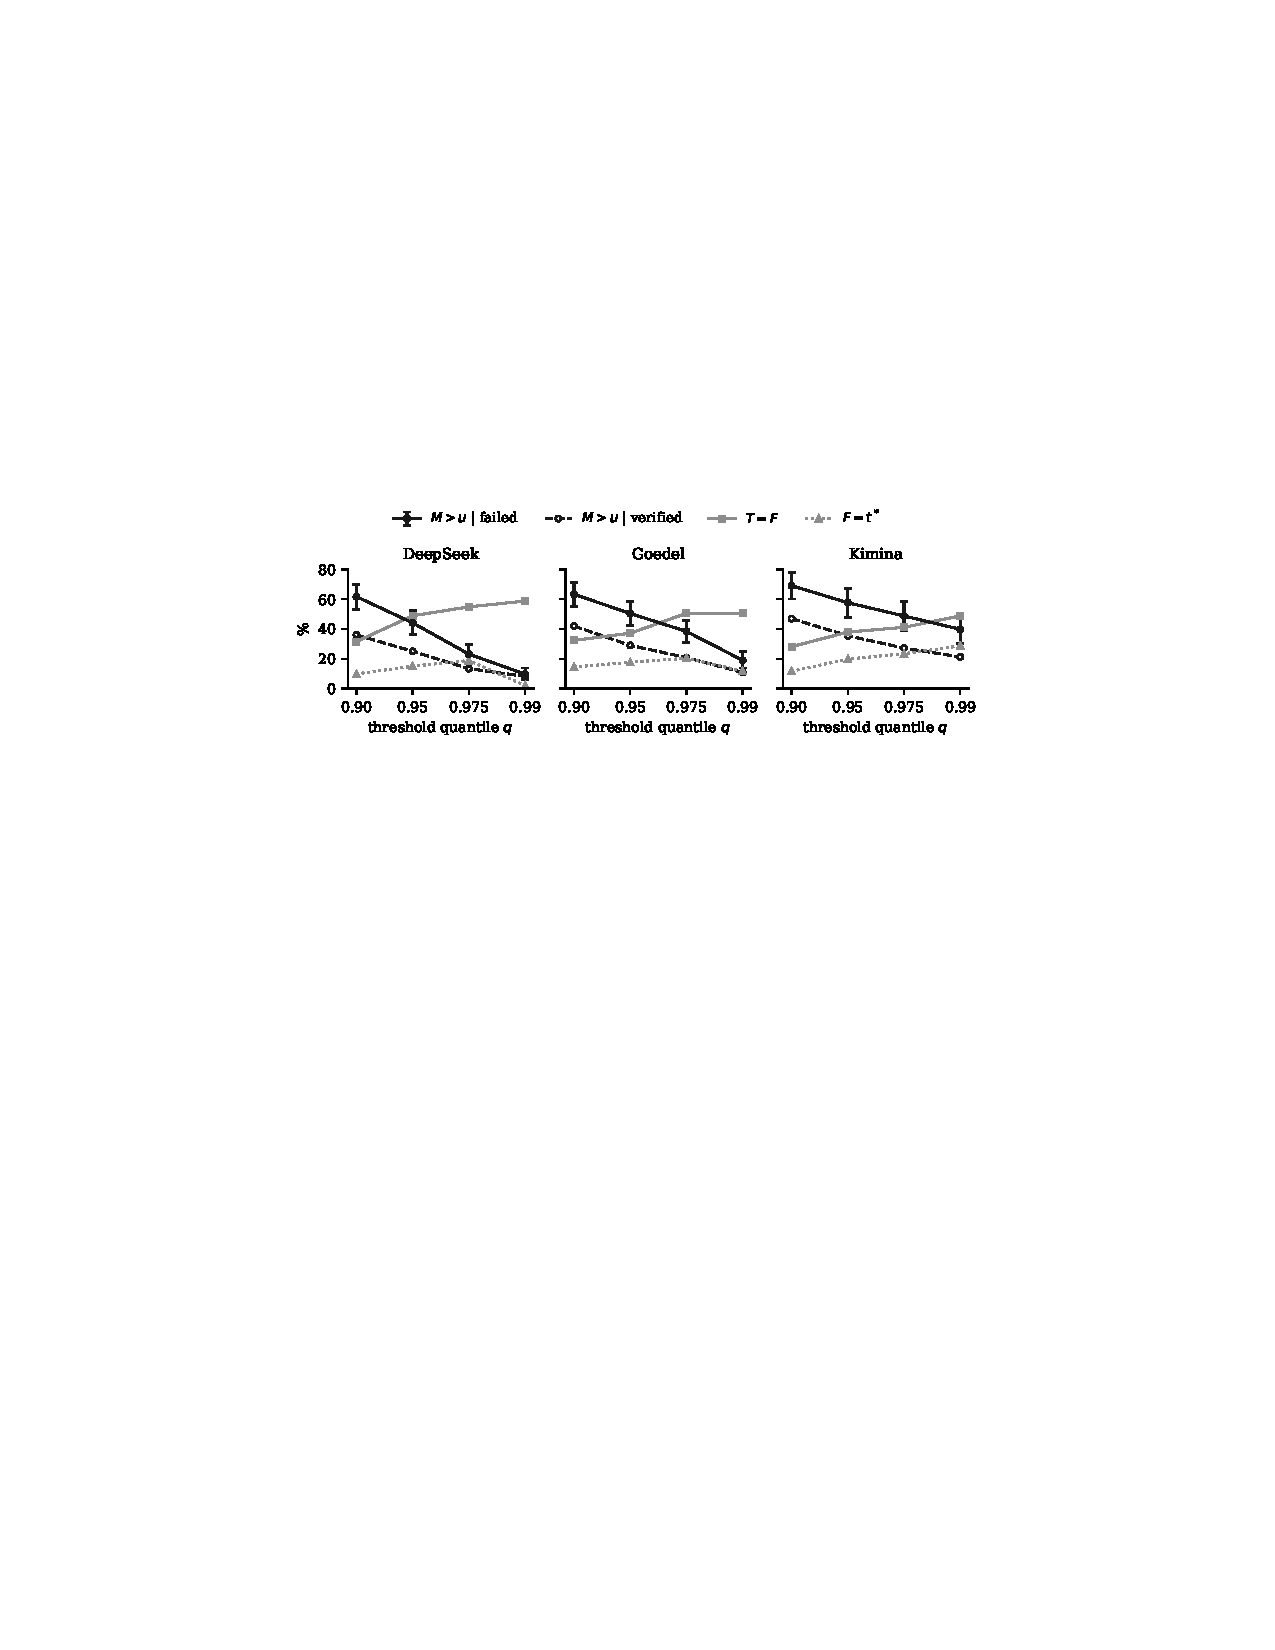
\includegraphics[width=0.95\linewidth]{fig_threshold.pdf}
\end{center}
\caption{Threshold diagnostics on miniF2F across quantiles $q$ of verified calibration increments. Failed proofs exceed the threshold more often than verified proofs of the same tasks (black), but the first exceedance rarely falls on the rejected step (grey dotted), and the maximum coincides with the first exceedance in only 28--59\% of cases (grey solid). Error bars: 95\% task-bootstrap intervals.}
\label{fig:threshold}
\end{figure}

\paragraph{Exceedance is more frequent in failed proofs but does not identify failure.} At $q=0.95$ on miniF2F, 44--58\% of failed proofs exceed the threshold against 25--35\% of verified proofs of the same tasks (Table~\ref{tab:threshold}), and the gap persists at every quantile (Figure~\ref{fig:threshold}). At no threshold does exceedance separate the two outcomes: failed proofs without an exceedance and verified proofs with one are both common.

\paragraph{Step-level coupling is the main loss; clustering is the second.} When a failed proof exceeds the threshold, its first exceedance is the rejected step in 15--20\% of miniF2F cases and 23--26\% on ProofNet at $q=0.95$, and never more than a third at any quantile. Clustering compounds this: the maximum coincides with the first exceedance in 37--49\% of miniF2F cases at $q=0.95$ and 49--59\% at $q=0.99$, so a later and larger step often follows the first one. Under the theorem's conditions both quantities would tend to one.

\paragraph{The absolute scale shifts across benchmarks.} With the whitening transform and thresholds calibrated on miniF2F, 85--88\% of failed and 63--75\% of verified ProofNet proofs exceed the $q=0.95$ threshold. The same fixed transform places ProofNet increments far higher, so a tolerance calibrated on one benchmark does not carry over to another. Together with Section~\ref{sec:loc}, these diagnostics locate the departure from Hypothesis~\ref{hyp:coupling} in its absolute tolerance: the rejected step is extreme \emph{relative to its own proof}, not beyond a common level.

\section{Online alarms}\label{sec:online}

A relative marker is hard to use online, where each step is judged before the rest of the proof exists. We fit a discrete hazard model on ProofNet: for failed attempts the steps $1,\dots,t^*$ enter with target $\1\{t=t^*\}$, and verified attempts of the same groups enter with all steps as survivors. The baseline H0 uses only past and present features (step index, $\log t$, span length, tactic category, surprisal and its running statistics); H1 adds $\log(1+w_t)$, the running maximum of $w$ and the ratio of $w_t$ to that maximum. Both use the nested group cross-validation of Section~\ref{sec:learned}. An alarm fires at the first step whose hazard exceeds a threshold set on inner out-of-fold verified attempts for a target false-alarm rate.

Online exact localization is 8--21\%, and the jump features change it by $-0.45$\,pp in the primary cell ($[-2.51, 1.86]$) and by $-4.47$ to $+1.63$\,pp elsewhere (Table~\ref{tab:online}, Appendix~\ref{app:temp}). Realized false-alarm rates depart from their targets (15.6\% at a 10\% target for DeepSeek): an alarm level calibrated on held-out verified proofs transfers imperfectly, as the threshold diagnostics of Section~\ref{sec:why} predict. Online, the jump adds nothing measurable to position and surprisal.


\section{Added value beyond cheap step features}\label{sec:learned}

\paragraph{Design.} We compare two independently fitted ridge-regularized conditional-logit localizers \citep{mcfadden1974}. For attempt $i$, each assigns a distribution over candidate steps,
\begin{equation}\label{eq:clogit}
p_{it}^{(m)}=\frac{\exp(r_{it}^{(m)})}{\sum_{s=1}^{L_i}\exp(r_{is}^{(m)})},\qquad r_{it}^{(0)}=\theta_0^\top\phi(b_{it}),\qquad r_{it}^{(1)}=\theta_1^\top\phi(b_{it})+\beta u_{it}.
\end{equation}
Baseline features are step index $t$, relative position $t/L_i$, first/last-step indicators, $\log(1+n_{it})$ for token-span length, AST tactic category and mean surprisal, with cubic B-splines for the four numeric features; $u_{it}$ is standardized $\log(1+w_{it})$ and $\beta$ is unconstrained in sign. The loss is the negative log-probability of $t_i^*$ with equal total weight per exercise group, under five outer and three inner group folds \citep{varma2006}; all preprocessing and the ridge parameter are fitted within training splits, and paired intervals resample whole groups 20,000 times on the saved out-of-fold predictions (Appendix~\ref{app:incremental}).


\paragraph{Results.} The learned localizer M0 is far stronger than any single signal (40.9\% and 57.8\% exact; Table~\ref{tab:learned}). For DeepSeek, the primary cell, adding the jump raises exact localization to 43.5\%, a gain of $+2.66$\,pp ($[0.45, 5.17]$; 97.5\% family interval $[0.25, 5.57]$), with 14 attempts corrected and 6 lost, concentrated in short proofs and first-step failures (Table~\ref{tab:strata}). For Goedel, exact localization changes by $-0.69$\,pp ($[-3.13, 1.57]$). With 133 groups this cell detects effects of about 3.4\,pp at 80\% power, so the change in exact localization is inconclusive; its out-of-fold NLL is worse by 0.056 nats ($[0.023, 0.092]$; Table~\ref{tab:incremental}, Appendix~\ref{app:incremental}). With M0 and M1 refitted on miniF2F at temperature 0.6 and frozen, the DeepSeek gain does not transfer to temperature-1.0 samples (Holm-adjusted one-sided $p=0.48$). The standardized jump coefficient is positive in every outer fold for both provers (0.11--0.42): conditional on position, span, tactic and surprisal, larger increments mark the first rejection.

\paragraph{Agreement with surprisal.} When the jump and surprisal maxima fall on the same or adjacent steps (23--45\% of eligible failures), the region of at most two steps contains the first rejection in 45--60\% of them, 1.4--2.0 times as often as a random window of the same size (Appendix~\ref{app:agreement}). Against single signals given the same number of candidates on proofs of the same length, all ten differences are positive (+2 to +17 points), and three exclude zero after Bonferroni correction over 40 contrasts. As a detector of failed proofs, agreement adds nothing to length. When two signals of different nature point to neighboring steps, the first failure lies there; this within-proof property carries no cross-proof information, as Section~\ref{sec:why} predicts.

\section{Other predictions of the framework}\label{sec:other}

\paragraph{Success versus length (P5).} Following Proposition~\ref{prop:length}, we test Qwen2.5-7B-Instruct \citep{qwen2024} on synthetic modus-ponens chains with distractors \citep{saparov2023}, with assigned lengths $L=3,\dots,12$, 1,000 calibration and 500 held-out tasks per temperature, and a symbolic checker. A one-parameter model $p_c(L)=\exp(-cL)$ fitted on calibration outcomes lowers held-out Brier score from 0.1398 to 0.1269 at temperature 1.0 ($c=0.268$), an improvement of 9.2\% (97.5\% interval $[0.0024, 0.0242]$ in absolute terms), and by 0.0065 ($[-0.0040, 0.0178]$) at 0.6. Success decays with length, but the exponential form is not specific: linear, Weibull, nonparametric and two further parametric models reach 0.1266--0.1274 at temperature 1.0, and the nonparametric model is best at 0.6 (0.1388 against 0.1424). The hazard of the first locally invalid inference also changes with step index (likelihood-ratio tests against a constant hazard, $p\le10^{-4}$; Appendix~\ref{app:dynamics}). Length is predictive, but the constant-hazard mechanism behind Proposition~\ref{prop:length} is not supported.

\paragraph{Tail behavior (P1, P3, P4).} No Pareto law appears at the first rejection (P3), consistent with the absence of a common threshold in Section~\ref{sec:why}. For P1, refuted-minus-verified moment-estimator contrasts have 95\% intervals $[-1.333, 0.754]$, $[-0.239, 0.141]$ and $[-0.995, 0.353]$ for DeepSeek, Goedel and Kimina (Appendix~\ref{app:tails}). The peak-to-neighbor ratio of the maximum shows no outcome effect after length and task adjustment. For P4, in five paired modular-addition trainings \citep{nanda2023}, signed tail estimates are nonpositive before and after the generalization transition and for shuffled-label controls. The supported content of the framework is its localization structure.

\section{Related work}

\paragraph{Extreme values and recurrences.} Tail processes describe dependence around large observations \citep{basrak2009,kulik2020}, and the extremal index links clustering to limits of maxima \citep{leadbetter1983}. Kesten--Goldie theory \citep{kesten1973,goldie1991,buraczewski2016} yields heavy tails of SGD iterates \citep{gurbuzbalaban2021,hodgkinson2021}; heavy tails also appear in gradient noise \citep{simsekli2019} and weight spectra \citep{martin2021}.

\paragraph{Error signals and formal reasoning.} Hidden-state probes detect falsehoods and hallucinations \citep{azaria2023,orgad2025}, semantic entropy detects confabulation \citep{farquhar2024}, and process supervision assesses individual reasoning steps \citep{lightman2024}. The provers we study generate verifiable Lean proofs \citep{ren2025,lin2025,wang2025}; compositionality studies model failure as compounding per-step error \citep{dziri2023,saparov2023}, and work on modular addition \citep{nanda2023} and heuristic arithmetic \citep{nikankin2025} motivates the algorithm/heuristic contrast behind the tail regimes.

\section{Discussion and conclusion}\label{sec:discussion}

One of the five predictions fixed in advance is confirmed: the largest residual change marks the first rejected step (P2). Within a proof the effect exceeds a positional control in every cell and survives changes of layer, shrinkage and calibration fold; across the full proof it exceeds the first-step rule on miniF2F and a fitted positional prior in some miniF2F cells, but not position on ProofNet. Success decays with length (P5), but not through the constant hazard the framework proposes. The three tail predictions (P1, P3, P4) fail.

The framework explains why the maximum misses. Its idealized limit requires that rejection coincide with crossing a fixed tolerance and that large steps not cluster. The data break the first condition most: failed proofs exceed a fixed level more often than verified ones, but the first exceedance rarely lands on the rejected step, and the scale shifts between benchmarks. Clustering is the second loss. What survives is extremality within a trace.

Appendix~\ref{app:protocol} specifies a confirmatory test of these results on new tasks.

\section*{Reproducibility statement}
Appendix~\ref{app:proofs} gives the proofs; Appendices~\ref{app:readout}--\ref{app:dynamics} and \ref{app:sensitivity} give read-out, segmentation, frozen revisions, the group-weighted objective, feature preprocessing, nested cross-validation, positional references, the prefix control, length models, read-out sensitivity and uncertainty procedures. The experimental archive fixes code and data by SHA256 before localizer fitting and records group splits, preprocessing parameters, coefficients, per-step out-of-fold predictions, per-group contrasts, bootstrap replicates and per-attempt exclusions. Reproduction additionally requires the prompts and the executable model and Lean environments. Appendix~\ref{app:protocol} gives the confirmatory protocol.

\section*{AI use statement}
AI tools assisted with manuscript editing and with checks of consistency between manuscript claims and reported experimental results.


\begin{thebibliography}{50}
\providecommand{\natexlab}[1]{#1}

\bibitem[Azaria \& Mitchell(2023)]{azaria2023}
Amos Azaria and Tom Mitchell.
\newblock The internal state of an {LLM} knows when it's lying.
\newblock In \emph{Findings of the Association for Computational Linguistics: EMNLP 2023}, 2023.

\bibitem[Azerbayev et~al.(2023)]{azerbayev2023}
Zhangir Azerbayev, Bartosz Piotrowski, Hailey Schoelkopf, Edward~W. Ayers, Dragomir Radev, and Jeremy Avigad.
\newblock {ProofNet}: Autoformalizing and formally proving undergraduate-level mathematics.
\newblock \emph{arXiv preprint arXiv:2302.12433}, 2023.

\bibitem[Basrak \& Segers(2009)]{basrak2009}
Bojan Basrak and Johan Segers.
\newblock Regularly varying multivariate time series.
\newblock \emph{Stochastic Processes and their Applications}, 119(4):1055--1080, 2009.

\bibitem[Breiman(1965)]{breiman1965}
Leo Breiman.
\newblock On some limit theorems similar to the arc-sin law.
\newblock \emph{Theory of Probability and its Applications}, 10(2):323--331, 1965.

\bibitem[Buraczewski et~al.(2016)]{buraczewski2016}
Dariusz Buraczewski, Ewa Damek, and Thomas Mikosch.
\newblock \emph{Stochastic Models with Power-Law Tails: The Equation $X = AX + B$}.
\newblock Springer, 2016.

\bibitem[de~Haan \& Ferreira(2006)]{dehaan2006}
Laurens de~Haan and Ana Ferreira.
\newblock \emph{Extreme Value Theory: An Introduction}.
\newblock Springer, 2006.

\bibitem[de~Moura \& Ullrich(2021)]{demoura2021}
Leonardo de~Moura and Sebastian Ullrich.
\newblock The {Lean} 4 theorem prover and programming language.
\newblock In \emph{Automated Deduction -- CADE 28}, 2021.

\bibitem[Dekkers et~al.(1989)]{dekkers1989}
Arnold L.~M. Dekkers, John H.~J. Einmahl, and Laurens de~Haan.
\newblock A moment estimator for the index of an extreme-value distribution.
\newblock \emph{Annals of Statistics}, 17(4):1833--1855, 1989.

\bibitem[Dziri et~al.(2023)]{dziri2023}
Nouha Dziri, Ximing Lu, Melanie Sclar, Xiang~Lorraine Li, Liwei Jiang, Bill~Yuchen Lin, Sean Welleck, Peter West, Chandra Bhagavatula, Ronan Le~Bras, Jena~D. Hwang, Soumya Sanyal, Xiang Ren, Allyson Ettinger, Za{\"i}d Harchaoui, and Yejin Choi.
\newblock Faith and fate: Limits of transformers on compositionality.
\newblock In \emph{Advances in Neural Information Processing Systems (NeurIPS)}, 2023.

\bibitem[Farquhar et~al.(2024)]{farquhar2024}
Sebastian Farquhar, Jannik Kossen, Lorenz Kuhn, and Yarin Gal.
\newblock Detecting hallucinations in large language models using semantic entropy.
\newblock \emph{Nature}, 630:625--630, 2024.

\bibitem[Geifman \& El-Yaniv(2019)]{geifman2019}
Yonatan Geifman and Ran El-Yaniv.
\newblock {SelectiveNet}: A deep neural network with an integrated reject option.
\newblock In \emph{Proceedings of the 36th International Conference on Machine Learning}, volume~97 of \emph{PMLR}, pp.\ 2151--2159, 2019.

\bibitem[Goldie(1991)]{goldie1991}
Charles~M. Goldie.
\newblock Implicit renewal theory and tails of solutions of random equations.
\newblock \emph{Annals of Applied Probability}, 1(1):126--166, 1991.

\bibitem[G{\"u}rb{\"u}zbalaban et~al.(2021)]{gurbuzbalaban2021}
Mert G{\"u}rb{\"u}zbalaban, Umut {\c{S}}im{\c{s}}ekli, and Lingjiong Zhu.
\newblock The heavy-tail phenomenon in {SGD}.
\newblock In \emph{International Conference on Machine Learning (ICML)}, 2021.

\bibitem[Hodgkinson \& Mahoney(2021)]{hodgkinson2021}
Liam Hodgkinson and Michael~W. Mahoney.
\newblock Multiplicative noise and heavy tails in stochastic optimization.
\newblock In \emph{International Conference on Machine Learning (ICML)}, 2021.

\bibitem[Kesten(1973)]{kesten1973}
Harry Kesten.
\newblock Random difference equations and renewal theory for products of random matrices.
\newblock \emph{Acta Mathematica}, 131:207--248, 1973.

\bibitem[Kulik \& Soulier(2020)]{kulik2020}
Rafa{\l} Kulik and Philippe Soulier.
\newblock \emph{Heavy-Tailed Time Series}.
\newblock Springer, 2020.

\bibitem[Kwon et~al.(2023)]{kwon2023}
Woosuk Kwon, Zhuohan Li, Siyuan Zhuang, Ying Sheng, Lianmin Zheng, Cody~Hao Yu, Joseph~E. Gonzalez, Hao Zhang, and Ion Stoica.
\newblock Efficient memory management for large language model serving with {PagedAttention}.
\newblock In \emph{Proceedings of the 29th Symposium on Operating Systems Principles (SOSP)}, 2023.

\bibitem[Leadbetter et~al.(1983)]{leadbetter1983}
M.~Ross Leadbetter, Georg Lindgren, and Holger Rootz{\'e}n.
\newblock \emph{Extremes and Related Properties of Random Sequences and Processes}.
\newblock Springer, 1983.

\bibitem[Lightman et~al.(2024)]{lightman2024}
Hunter Lightman, Vineet Kosaraju, Yuri Burda, Harrison Edwards, Bowen Baker, Teddy Lee, Jan Leike, John Schulman, Ilya Sutskever, and Karl Cobbe.
\newblock Let's verify step by step.
\newblock In \emph{International Conference on Learning Representations (ICLR)}, 2024.

\bibitem[Lin et~al.(2025)]{lin2025}
Yong Lin, Shange Tang, Bohan Lyu, Ziran Yang, Jui-Hui Chung, Haoyu Zhao, Lai Jiang, Yihan Geng, Jiawei Ge, Jingruo Sun, Jiayun Wu, Jiri Gesi, David Acuna, Kaiyu Yang, Hongzhou Lin, Yejin Choi, Danqi Chen, Sanjeev Arora, and Chi Jin.
\newblock {Goedel-Prover-V2}: Scaling formal theorem proving with scaffolded data synthesis and self-correction.
\newblock \emph{arXiv preprint arXiv:2508.03613}, 2025.

\bibitem[Martin \& Mahoney(2021)]{martin2021}
Charles~H. Martin and Michael~W. Mahoney.
\newblock Implicit self-regularization in deep neural networks: Evidence from random matrix theory and implications for learning.
\newblock \emph{Journal of Machine Learning Research}, 22(165):1--73, 2021.

\bibitem[McFadden(1974)]{mcfadden1974}
Daniel McFadden.
\newblock Conditional logit analysis of qualitative choice behavior.
\newblock In P.~Zarembka (ed.), \emph{Frontiers in Econometrics}, pp.\ 105--142. Academic Press, 1974.

\bibitem[Nanda et~al.(2023)]{nanda2023}
Neel Nanda, Lawrence Chan, Tom Lieberum, Jess Smith, and Jacob Steinhardt.
\newblock Progress measures for grokking via mechanistic interpretability.
\newblock In \emph{International Conference on Learning Representations (ICLR)}, 2023.

\bibitem[Nikankin et~al.(2025)]{nikankin2025}
Yaniv Nikankin, Anja Reusch, Aaron Mueller, and Yonatan Belinkov.
\newblock Arithmetic without algorithms: Language models solve math with a bag of heuristics.
\newblock In \emph{International Conference on Learning Representations (ICLR)}, 2025.

\bibitem[Orgad et~al.(2025)]{orgad2025}
Hadas Orgad, Michael Toker, Zorik Gekhman, Roi Reichart, Idan Szpektor, Hadas Kotek, and Yonatan Belinkov.
\newblock {LLMs} know more than they show: On the intrinsic representation of {LLM} hallucinations.
\newblock In \emph{International Conference on Learning Representations (ICLR)}, 2025.

\bibitem[Pickands(1975)]{pickands1975}
James Pickands.
\newblock Statistical inference using extreme order statistics.
\newblock \emph{Annals of Statistics}, 3(1):119--131, 1975.

\bibitem[Qwen Team(2024)]{qwen2024}
Qwen Team.
\newblock {Qwen2.5} technical report.
\newblock \emph{arXiv preprint arXiv:2412.15115}, 2024.

\bibitem[Ren et~al.(2025)]{ren2025}
Z.~Z. Ren, Zhihong Shao, Junxiao Song, Huajian Xin, Haocheng Wang, Wanjia Zhao, Liyue Zhang, Zhe Fu, Qihao Zhu, Dejian Yang, Z.~F. Wu, Zhibin Gou, Shirong Ma, Hongxuan Tang, Yuxuan Liu, Wenjun Gao, Daya Guo, and Chong Ruan.
\newblock {DeepSeek-Prover-V2}: Advancing formal mathematical reasoning via reinforcement learning for subgoal decomposition.
\newblock \emph{arXiv preprint arXiv:2504.21801}, 2025.

\bibitem[Resnick(1987)]{resnick1987}
Sidney~I. Resnick.
\newblock \emph{Extreme Values, Regular Variation, and Point Processes}.
\newblock Springer, 1987.

\bibitem[Resnick(2007)]{resnick2007}
Sidney~I. Resnick.
\newblock \emph{Heavy-Tail Phenomena: Probabilistic and Statistical Modeling}.
\newblock Springer, 2007.

\bibitem[Saparov \& He(2023)]{saparov2023}
Abulhair Saparov and He~He.
\newblock Language models are greedy reasoners: A systematic formal analysis of chain-of-thought.
\newblock In \emph{International Conference on Learning Representations (ICLR)}, 2023.

\bibitem[{\c{S}}im{\c{s}}ekli et~al.(2019)]{simsekli2019}
Umut {\c{S}}im{\c{s}}ekli, Levent Sagun, and Mert G{\"u}rb{\"u}zbalaban.
\newblock A tail-index analysis of stochastic gradient noise in deep neural networks.
\newblock In \emph{International Conference on Machine Learning (ICML)}, 2019.

\bibitem[Sun et~al.(2024)]{sun2024}
Mingjie Sun, Xinlei Chen, J.~Zico Kolter, and Zhuang Liu.
\newblock Massive activations in large language models.
\newblock In \emph{Conference on Language Modeling (COLM)}, 2024.

\bibitem[Varma \& Simon(2006)]{varma2006}
Sudhir Varma and Richard Simon.
\newblock Bias in error estimation when using cross-validation for model selection.
\newblock \emph{BMC Bioinformatics}, 7:91, 2006.

\bibitem[Wang et~al.(2025)]{wang2025}
Haiming Wang, Mert Unsal, Xiaohan Lin, Mantas Baksys, Junqi Liu, Marco~Dos Santos, Flood Sung, Marina Vinyes, Zhenzhe Ying, Zekai Zhu, et~al.
\newblock {Kimina-Prover} preview: Towards large formal reasoning models with reinforcement learning.
\newblock \emph{arXiv preprint arXiv:2504.11354}, 2025.

\bibitem[Zheng et~al.(2022)]{zheng2022}
Kunhao Zheng, Jesse~Michael Han, and Stanislas Polu.
\newblock {miniF2F}: A cross-system benchmark for formal {Olympiad}-level mathematics.
\newblock In \emph{International Conference on Learning Representations (ICLR)}, 2022.

\end{thebibliography}


\clearpage
\appendix
\section{Proofs and full estimation assumptions}\label{app:proofs}

\subsection{Overshoots and the failure--length law}

For Proposition~\ref{prop:overshoot}, $Q_u(y)=\Fbar(uy)/\Fbar(u)$, so the claims for regularly and rapidly varying laws follow from the definitions. If $0<x_F<\infty$, then $1<Z/u\le x_F/u$ given $Z>u$, and the upper bound tends to one. Unbounded Gumbel-domain laws are a standard rapidly varying case \citep{dehaan2006,resnick1987}: their auxiliary function $f$ satisfies $f(u)/u\to0$ and $\Fbar(u+xf(u))/\Fbar(u)\to e^{-x}$. For fixed $y>1$ and $M>0$, eventually $(y-1)u\ge Mf(u)$, so $\limsup\Fbar(uy)/\Fbar(u)\le e^{-M}$; let $M\to\infty$.

For Proposition~\ref{prop:length}, coupling identifies $\{V_L=0\}$ with $\{M_L>\tau_L\}$, and the extremal-index limit gives the formula; the small-$\lambda$ statement is a Taylor expansion of the limit. The two approximations are logically separate: the joint high-threshold, long-window limit comes first, and only its limiting expression is expanded. Neither implies an exact fixed-threshold exponential law.

\subsection{Proof of conditional localization}

Let $A_t=\{Z_t>\tau,\ Z_s\le\tau\text{ for }s<t\}$. These disjoint events partition $\{M_L>\tau\}$, and coupling gives $t^*=t$ on $A_t$. For a regularly varying sequence, stationarity and~\eqref{eq:tail} give
\begin{align}
\PP(A_t)/\Fbar(\tau)&\to q_t=\PP(Y\Theta_{s-t}\le1\text{ for }s<t),\label{eq:qt}\\
\PP(A_t,T=t)/\Fbar(\tau)&\to r_t=\PP(Y\Theta_{s-t}\le1\text{ for }s<t,\ \Theta_{s-t}<1\text{ for }s>t).\label{eq:rt}
\end{align}
The past boundaries have probability zero because $Y$ is continuous and independent of $\Theta$, and $\PP(\Theta_j=1)=0$ removes the future ones. Thus the conditional probability tends to $\sum_tr_t/\sum_tq_t$. The denominator is at least $q_1=1$, $0\le r_t\le q_t$, and $r_1=\PP(\Theta_j<1,\ 1\le j<L)$ gives the positivity criterion. With atoms at one, the Portmanteau theorem applied to strict and non-strict future inequalities gives the bounds. This proves part (i) of Theorem~\ref{thm:loc}.

Under extremal independence and fixed $L$, $\PP(N_\tau\ge2)\le\sum_{s<t}\PP(Z_s>\tau,Z_t>\tau)=o(\Fbar(\tau))$. Also $\PP(A_t)=\Fbar(\tau)(1+o(1))$ and $\PP(M_L>\tau)=L\Fbar(\tau)(1+o(1))$. Conditional on failure there is exactly one exceedance with probability tending to one; it is both the first rejection and the global maximum, and each position has limiting probability $1/L$. For $y\ge1$,
\begin{equation}\label{eq:overshootloc}
\PP(Z_{t^*}>\tau y\mid V_L=0)=\frac{L\Fbar(\tau y)+o(\Fbar(\tau))}{L\Fbar(\tau)+o(\Fbar(\tau))},
\end{equation}
and regular or rapid variation completes part (ii).

\subsection{Proof of the scalar multiplier mechanism}\label{app:kesten}

Put $\Pi_{t,0}=1$ and $\Pi_{t,j}=a_t\cdots a_{t-j+1}$. The strong law gives $\Pi_{t,j}^{1/j}\to e^{\EE\log a}<1$ a.s., and Gaussian innovations grow subexponentially a.s.\ by Borel--Cantelli, so $E_t=\sum_{j\ge0}\Pi_{t,j}B_{t-j}$ converges absolutely, solves the recurrence and is its stationary causal solution; uniqueness follows from contraction of the products \citep{buraczewski2016}. Conditional on the multipliers, $E_t$ is Gaussian with covariance $R_t\Sigma$, where $R_t=\sum_{j\ge0}\Pi_{t,j}^2=a_t^2R_{t-1}+1$.

\paragraph{Heavy tails.} Goldie's renewal theorem \citep{goldie1991} with multiplier $a^2$ and exponent $\alpha/2$ gives $\PP(R_t>x)\sim C_Rx^{-\alpha/2}$, $C_R>0$; the moment condition implies $\EE a^\alpha\log^+a<\infty$, and the renewal condition is assumed. Since $E_t\overset{d}{=}\sqrt{R_t}\,G$ with $G\sim\mathcal N(0,\Sigma)$ independent of $R_t$, Breiman's lemma \citep{breiman1965} gives $\PP(\|E_t\|>x)\sim C_R\EE\|G\|^\alpha x^{-\alpha}$. Next $E_t-E_{t-1}=(a_t-1)E_{t-1}+B_t$ with $a_t$ independent of $E_{t-1}$, and the same lemma applies because $\EE|a-1|^{\alpha+\delta}<\infty$. Light perturbations do not change the asymptotic: if $\|V\|$ is regularly varying and $\PP(\|W\|>\varepsilon x)=o(\PP(\|V\|>x))$, the triangle inequality places $\PP(\|V+W\|>x)/\PP(\|V\|>x)$ between $(1+\varepsilon)^{-\alpha}+o(1)$ and $(1-\varepsilon)^{-\alpha}+o(1)$; letting $\varepsilon\downarrow0$ covers the Gaussian term and bounded reference increments.

\paragraph{Light tails.} If $a\le\rho<1$, then $R_{t-1}\le(1-\rho^2)^{-1}$ and, conditional on the multipliers, the increment has covariance $s_t^2\Sigma$ with $s_t^2=1+(a_t-1)^2R_{t-1}\in[1,(2-\rho^2)/(1-\rho^2)]$. Gaussian concentration for $\|G\|$, with $G\sim\mathcal N(0,\Sigma)$ and $s_\rho^2=(2-\rho^2)/(1-\rho^2)$, gives $\PP(\|E_t-E_{t-1}\|>x)\le\exp\{-(x/s_\rho-\EE\|G\|)_+^2/(2\|\Sigma\|_{\mathrm{op}})\}$ and all moments. For rapid variation, let $\psi(u)=\PP(\|G\|>u)$; a one-coordinate Gaussian lower bound along a top eigenvector and the concentration upper bound give $\psi(uy)/\psi(u)\to0$ for $y>1$, hence $\EE\psi(xy/s_t)/\EE\psi(x/s_t)\le\sup_{u\ge x/s_\rho}\psi(uy)/\psi(u)\to0$.

\paragraph{Moment index and the two-point example.} Suppose $a$ has all positive moments. Since $\|E_t\|\overset{d}{=}\sqrt{R_t}\|G\|$, $\EE\|E_t\|^s<\infty$ iff $\EE R_t^{s/2}<\infty$. If $\EE a^s<1$, subadditivity ($s\le2$) or Minkowski's inequality ($s>2$) bounds this moment by a geometric series; if $\EE a^s>1$, $R_t\ge\Pi_{t,j}^2$ gives $\EE R_t^{s/2}\ge(\EE a^s)^j\to\infty$. When $\PP(a>1)>0$ and $\EE\log a<0$, convexity of $s\mapsto\log\EE a^s$ gives a unique positive root $\alpha$, the moment index; if $a\le1$ a.s., all moments exist. The increment has the same moment index by the triangle and reverse triangle inequalities. For the two-point law, $g_p(s)=(1-p)\rho^s+p\kappa^s-1$ is strictly convex, vanishes at zero and has negative slope there exactly when $p<p_c$, so it has a unique positive root on that range. Since $\partial_pg_p(s)=\kappa^s-\rho^s>0$, the root decreases strictly and continuously in $p$; as $p\downarrow0$, $\alpha(p)\to\infty$ and $p\kappa^{\alpha(p)}\to1$, so $\alpha(p)\sim\log(1/p)/\log\kappa$; as $p\uparrow p_c$, the slope at zero vanishes and strict convexity forces $\alpha(p)\downarrow0$. These statements need no non-arithmetic condition, which is required only for the exact power-tail constant.

\subsection{Pooled-trace estimation: consistency and a normal limit}\label{app:hill}

Let $Z^{(1)},\dots,Z^{(m)}$ be i.i.d.\ traces of fixed length $L$ with arbitrary within-trace dependence, average marginal survival $\Fbar(x)=L^{-1}\sum_{t\le L}\PP(Z_t>x)$ and pooled sample size $n=mL$. The Hill estimator on the pooled descending order statistics is $\hat\gamma_k^H=k^{-1}\sum_{j\le k}\log(Z_{(j)}/Z_{(k+1)})$.

\begin{theorem}[Pooled-trace consistency]\label{thm:hill}
If $\Fbar\in RV_{-\alpha}$, $k\to\infty$ and $k/n\to0$, then $\hat\gamma_k^H\to1/\alpha$ in probability for fixed $L$, without any condition on dependence within a trace.
\end{theorem}

\begin{proof}
Let $b=b(n/k)$ be the upper quantile of the average marginal law, so $(n/k)\Fbar(b)\to1$, and define $\nu_m=k^{-1}\sum_{j\le m}\sum_{t\le L}\delta_{Z_t^{(j)}/b}$. For bounded continuous $f$ supported in $[y_0,\infty]$, $y_0>0$, the expectation of $\nu_m(f)$ tends to its integral under $\nu_\alpha(y,\infty]=y^{-\alpha}$. A trace contributes at most $L$ points; if it contributes $N$, then $N^2\le LN$, and independence across traces gives
\begin{equation}\label{eq:varnu}
\operatorname{Var}\nu_m(f)\le\|f\|_\infty^2\,\frac{L}{k}\cdot\frac{n\PP(Z\ge by_0)}{k}\to0,
\end{equation}
where $Z$ has the average marginal law. The pooled tail empirical measure therefore converges in probability under arbitrary within-trace dependence. Quantile bracketing at $b(1\pm\varepsilon)$ gives $Z_{(k+1)}/b\to1$, and $\hat\gamma_k^H=\int_1^\infty\nu_m(yZ_{(k+1)}/b,\infty]\,dy/y$. Monotonicity and continuity of the limit give uniform convergence on compact $y$-intervals; on the bracketing event a Potter bound with $0<\eta<\alpha$ bounds the expected remainder beyond $M$ by a constant times $\int_M^\infty y^{-\alpha+\eta-1}dy\to0$. Hence $\hat\gamma_k^H\to\int_1^\infty y^{-\alpha-1}dy=1/\alpha$ \citep{resnick2007}.
\end{proof}

\begin{theorem}[Conditional normal limit for pooled Hill estimation]\label{thm:hillclt}
In the setting of Theorem~\ref{thm:hill}, put $\gamma=1/\alpha$ and assume the average marginal law is continuous in its upper tail. Suppose its upper quantile $U$ satisfies second-order regular variation, $\{U(tx)/U(t)-x^\gamma\}/A(t)\to x^\gamma(x^{\rho_2}-1)/\rho_2$ with $\rho_2\le0$ (logarithmic limit at $\rho_2=0$), $A(t)\to0$ and $\sqrt kA(n/k)\to\lambda\in\mathbb R$. Suppose
\begin{equation}\label{eq:sigmacl}
\sigma_{\mathrm{cl}}^2=\lim_{x\to\infty}\frac{\operatorname{Var}\bigl(\sum_{t\le L}g_x(Z_t)\bigr)}{\gamma^2L\Fbar(x)}\in(0,\infty),\qquad g_x(z)=\log^+(z/x)-\gamma\1\{z>x\}.
\end{equation}
With $b$ chosen so that $n\Fbar(b)=k$, assume local stochastic equicontinuity at one of $W_m(y)=\sqrt k\{k^{-1}\sum_{j,t}\1\{Z_t^{(j)}>by\}-(n/k)\Fbar(by)\}$: for every $\varepsilon>0$, $\lim_{\delta\downarrow0}\limsup_m\PP(\sup_{|y-1|\le\delta}|W_m(y)-W_m(1)|>\varepsilon)=0$. Then $\sqrt k(\hat\gamma_k^H-\gamma)\Rightarrow\mathcal N(\lambda/(1-\rho_2),\gamma^2\sigma_{\mathrm{cl}}^2)$. For independent steps within a trace, $\sigma_{\mathrm{cl}}^2=1$.
\end{theorem}

\begin{proof}
Let $Y_j=\sum_tg_b(Z_t^{(j)})$, let $\tilde\gamma_b$ be the ratio of pooled $\log^+(Z/b)$ to the pooled number of exceedances of $b$, and $N_m(y)=\nu_m(y,\infty]$. Then $\sqrt k(\tilde\gamma_b-\gamma)=k^{-1/2}\sum_jY_j/N_m(1)$, and the denominator tends to one. The second-order condition gives the usual bias $\sqrt k(m/k)\EE Y_1\to\lambda/(1-\rho_2)$, since expectations depend only on the average marginal law \citep{dehaan2006}. The numerator variance tends to $\gamma^2\sigma_{\mathrm{cl}}^2$. For Lindeberg, $|Y_1|\le L(\log^+(\max_tZ_t/b)+\gamma)\1\{\max_tZ_t>b\}$ and regular variation give $\EE Y_1^4=O(L^5\Fbar(b))$, so $(m/k)\EE[Y_1^2\1\{|Y_1|>\varepsilon\sqrt k\}]\to0$ for fixed $L$, and the triangular-array CLT gives the deterministic-threshold limit.

Put $q_m=Z_{(k+1)}/b$ and $I_m(q)=\int_q^\infty N_m(y)\,dy/y$. Since $N_m(1)-1=O_p(k^{-1/2})$, local equicontinuity and the deterministic derivative $-\alpha$ at one give $q_m-1=\gamma\{N_m(1)-1\}+o_p(k^{-1/2})$, after quantile bracketing establishes tightness at this scale. Ties involve at most $L$ observations a.s.\ and contribute $O(L/k)=o(k^{-1/2})$. Hence $\hat\gamma_k^H=I_m(1)-\gamma\{N_m(1)-1\}+o_p(k^{-1/2})$, the same expansion as $\tilde\gamma_b=I_m(1)/N_m(1)$. For independent coordinates the variance is a sum of marginal variances and $\sigma_{\mathrm{cl}}^2=1$; otherwise covariance terms remain.
\end{proof}

Local equicontinuity is a separate assumption, not a consequence of the scalar variance limit.

\section{Read-out, segmentation and frozen revisions}\label{app:readout}

DeepSeek has 30 decoder blocks and Goedel and Kimina 36; all read-outs have dimension 4,096. The archived quarter/middle/three-quarter layers are 6/14/21 (DeepSeek) and 8/17/26 (Goedel, Kimina); the middle layer is the principal evaluation, and Appendix~\ref{app:sensitivity} repeats the localization analyses at the other two. The formal-entry anchor is the last original token ending at the start of the formal proof body, allowing only trailing whitespace. Moving the anchor changes the first raw increment, and refitting the transform can change all whitened scores. The formal-entry analysis fixes calibration fold 0 and shrinkage 0.1; no evaluation labels enter the transform. Semantic replay and token alignment must agree on the first reproducible rejection; unresolved localization, parse failures and resource failures are kept distinct from localizable rejection. Kimina's processing removes terminal text after proof completion.

\begin{table}[h]
\caption{Frozen model revisions and benchmark snapshots.}
\label{tab:revisions}
\begin{center}
\small
\begin{tabular}{ll}
\toprule
Artifact & Revision\\
\midrule
DeepSeek-Prover-V2-7B & \texttt{a8d9e14432b2e8dd9df2a4d4e70f1ba9bc8d9b7b}\\
Goedel-Prover-V2-8B & \texttt{dfd02e6271a58375dfbf3ece0175277cf6b6a89a}\\
Kimina-Prover-Distill-8B & \texttt{74d328a7b1f001ab4871812582fc66d9bf70c68b}\\
miniF2F (Lean 4) & \texttt{70a1249ce240667f6bcdd1ccd62f847f0e065d57}\\
ProofNet-Verified & \texttt{160414332dc196583f6c37c310b420d2a3b07c58}\\
\bottomrule
\end{tabular}
\end{center}
\end{table}

\section{Incremental-analysis protocol and supplementary results}\label{app:incremental}

\paragraph{Population, labels and features.} The comparison retains attempts with $L\ge2$, complete token boundaries and reliable semantic replay; ambiguous localization, parse errors and missing replay exclude the whole attempt, and no candidate step is dropped. The AST fixes candidate boundaries before execution, the diagnostic is mapped to a node, and prefix and rejection are reproduced in saved local contexts. A training label zero means ``not the first rejection'', not ``verified correct'', which differs from the absorbing labels of Section~\ref{sec:theory}. The numeric features $t$, $t/L$, $\log(1+n_{\mathrm{tokens}})$ and mean surprisal use cubic B-splines with four training-quantile knots (linear fallback when knots coincide; constant extrapolation). Categories in fewer than ten training groups, and unseen ones, map to \texttt{OTHER}. No intercept or raw $L$ is added, since attempt-constant scores cancel in the softmax; relative position still lets scores depend on length.

\paragraph{Objective and cross-validation.} With $G$ training groups, $n_g$ attempts in group $g$ and $\ell_{im}=\log\sum_{t\le L_i}e^{r_{it}^{(m)}}-r_{it_i^*}^{(m)}$, each model minimizes
\begin{equation}\label{eq:objective}
\mathcal L_m=\frac1G\sum_g\frac1{n_g}\sum_{i\in g}\ell_{im}+\frac\lambda2\|\eta_m\|_2^2,
\end{equation}
with no division by $L_i$ and no class reweighting; preprocessing row weights are $1/(Gn_{g(i)}L_i)$. Five outer group folds; within each, three inner folds choose $\lambda\in\{10^{-4},\dots,10\}$ (decades) by pooled inner-validation equal-group NLL, ties within $10^{-10}$ favoring the larger penalty. Scalers, knots and category maps are refitted on each training split. The chosen $\lambda$ is 0.1 throughout except M1 in one Goedel fold ($\lambda=1$). All 190 optimizations per prover converged with $\max|\nabla|<2\times10^{-5}$. Metrics are $H_m=G^{-1}\sum_gn_g^{-1}\sum_{i\in g}\1\{\hat t_i^{(m)}=t_i^*\}$, $\Delta H=H_1-H_0$ and $\Delta\mathrm{NLL}=G^{-1}\sum_gn_g^{-1}\sum_{i\in g}(\ell_{i0}-\ell_{i1})$; the $\pm1$ metric uses $\1\{|\hat t-t^*|\le1\}$.

\paragraph{Uncertainty and sample support.} Twenty thousand bootstrap replicates sample whole groups, identical for both models, without refitting; 95\% percentile intervals plus 97.5\% intervals for the two-cell family. The 97.5\% family intervals for $\Delta$NLL are $[-0.0064, 0.0237]$ (DeepSeek) and $[-0.0967, -0.0180]$ (Goedel). Standardized jump coefficients by outer fold are 0.208, 0.171, 0.231, 0.200, 0.248 (DeepSeek) and 0.211, 0.246, 0.418, 0.251, 0.111 (Goedel); these come from overlapping training sets and are not independent tests. A fixed-fit calculation gives a group standard error of about 1.20\,pp and roughly 209/167 groups for 80\% power at 5\% against the +3\,pp target, compared with 166/133 available. The same calculation gives a Goedel group standard error of about 1.20\,pp at 133 groups, hence a minimum detectable effect of about 3.4\,pp at 80\% power and two-sided level 0.05 (Section~\ref{sec:learned}).

\begin{table}[h]
\caption{Incremental effect of the jump on ProofNet (equal group weights). $\Delta H=H_1-H_0$ in percentage points; $\Delta\mathrm{NLL}=\mathrm{NLL}_0-\mathrm{NLL}_1$ in nats, positive favors M1. 95\% paired group-bootstrap intervals.}
\label{tab:incremental}
\begin{center}
\small
\setlength{\tabcolsep}{4pt}
\begin{tabular}{lrrrcrc}
\toprule
Cell & $H_0$ & $H_1$ & $\Delta H$ & 95\% interval & $\Delta$NLL & 95\% interval\\
\midrule
DeepSeek (primary) & 40.85 & 43.51 & $+2.66$ & $[0.45, 5.17]$ & $+0.009$ & $[-0.004, 0.022]$\\
Goedel (replication) & 57.82 & 57.13 & $-0.69$ & $[-3.13, 1.57]$ & $-0.056$ & $[-0.092, -0.023]$\\
\bottomrule
\end{tabular}
\end{center}
\end{table}

\begin{table}[h]
\caption{Paired exact outcomes (attempt counts / equal-group shares) and mean absolute error.}
\label{tab:paired}
\begin{center}
\small
\begin{tabular}{lccccc}
\toprule
Model & Both correct & M1 only & M0 only & Both miss & MAE M0$\to$M1\\
\midrule
DeepSeek & 191 / 39.8\% & 14 / 3.7\% & 6 / 1.0\% & 241 / 55.5\% & 3.29 $\to$ 3.23\\
Goedel & 148 / 55.7\% & 5 / 1.4\% & 6 / 2.1\% & 100 / 40.7\% & 3.01 $\to$ 3.10\\
\bottomrule
\end{tabular}
\end{center}
\end{table}

\begin{table}[h]
\caption{Prespecified descriptive strata ($\Delta H$, pp). Groups can appear in several strata. No eligible proof in this population first fails at its last step.}
\label{tab:strata}
\begin{center}
\small
\begin{tabular}{llrrr}
\toprule
Model & Stratum & Attempts & Groups & $\Delta H$\\
\midrule
DeepSeek & $L=2$--10 & 188 & 83 & $+3.01$\\
DeepSeek & $L=11$--24 & 148 & 92 & 0.00\\
DeepSeek & $L\ge25$ & 116 & 68 & $+0.86$\\
DeepSeek & first-step failure & 99 & 49 & $+5.10$\\
DeepSeek & interior failure & 353 & 148 & $+1.69$\\
Goedel & $L=2$--10 & 120 & 64 & $+0.91$\\
Goedel & $L=11$--24 & 76 & 53 & $-0.31$\\
Goedel & $L\ge25$ & 63 & 48 & $-1.39$\\
Goedel & first-step failure & 83 & 49 & $-0.68$\\
Goedel & interior failure & 176 & 105 & $-0.32$\\
\bottomrule
\end{tabular}
\end{center}
\end{table}

\begin{table}[h]
\caption{Examples selected by smallest SHA256 trace ID within each prover/outcome class.}
\label{tab:examples}
\begin{center}
\small
\begin{tabular}{lllccc}
\toprule
Model & Outcome & Exercise & $t^*/L$ & M0 & M1\\
\midrule
DeepSeek & helped & Dummit--Foote 1.1.34 & 7/25 & 1 & 7\\
DeepSeek & harmed & Artin 10.2.4 & 6/42 & 6 & 1\\
DeepSeek & unchanged & Rudin 5.5 & 4/50 & 9 & 9\\
Goedel & helped & Rudin 2.28 & 1/4 & 3 & 1\\
Goedel & harmed & Dummit--Foote 1.1.5 & 9/16 & 9 & 2\\
Goedel & unchanged & Artin 2.4.19 & 2/12 & 2 & 2\\
\bottomrule
\end{tabular}
\end{center}
\end{table}

\section{Temperature-1.0 replication, controls and threshold diagnostics}\label{app:temp}

\paragraph{Temperature 1.0.} Eligibility, the formal-entry transform (calibration fold 0, shrinkage 0.1), the argmax localizers and M0/M1 (refitted once on temperature-0.6 miniF2F failures) were frozen before evaluation. Seven one-sided hypotheses were tested with Holm correction: Ha, exact jump argmax above uniform (three provers); Hb, $\pm1$ jump argmax above $\pm1$ surprisal argmax (three provers); Hc, M1 above M0 for DeepSeek. Tests use one-sided cluster-$t$ approximations over tasks; intervals use 20,000 task-bootstrap replicates. For DeepSeek, Hc has Holm-adjusted $p=0.479$.

\begin{table}[h]
\caption{Temperature-1.0 miniF2F evaluation with frozen rules (\%). $p$: Holm-adjusted over seven hypotheses.}
\label{tab:temp}
\begin{center}
\small
\begin{tabular}{lrrrrrrrr}
\toprule
Model & N/tasks & Jump & Uniform & Surprisal & Jump $\pm1$ & Surpr.\ $\pm1$ & $p$ (Ha) & $p$ (Hb)\\
\midrule
DeepSeek & 544/140 & 20.40 & 10.31 & 15.99 & 40.07 & 39.34 & $4.2\times10^{-4}$ & 0.547\\
Goedel & 456/124 & 20.18 & 9.11 & 14.04 & 36.40 & 34.21 & $1.9\times10^{-4}$ & 0.547\\
Kimina & 498/122 & 19.08 & 10.72 & 12.05 & 35.14 & 24.90 & $6.1\times10^{-4}$ & 0.0021\\
\bottomrule
\end{tabular}
\end{center}
\end{table}

\paragraph{Positional references.} The first-step rule predicts $\hat t=1$. The positional prior is a localizer fitted only on first-rejection positions of calibration failures: on miniF2F it is fitted once on temperature-0.6 calibration tasks and applied unchanged at temperature 1.0; on ProofNet it is cross-fitted over five exercise-group folds. Bootstrap intervals resample whole tasks (groups) with the fitted priors held fixed. Table~\ref{tab:positional} gives exact localization under both weightings.

\begin{table}[h]
\caption{Exact localization against positional references (\%). Jump$-$Prior in percentage points with 95\% task/group bootstrap intervals. Attempt: equal attempt weights (as in Table~\ref{tab:main}); Group: equal task (group) weights.}
\label{tab:positional}
\begin{center}
\scriptsize
\setlength{\tabcolsep}{1.8pt}
\begin{tabular}{lrrrrcrrrc}
\toprule
& \multicolumn{5}{c}{Attempt} & \multicolumn{4}{c}{Group}\\
\cmidrule(lr){2-6}\cmidrule(lr){7-10}
Cell & First & Prior & Jump & Surpr. & Jump$-$Prior & First & Prior & Jump & Jump$-$Prior\\
\midrule
miniF2F DeepSeek 0.6 & 7.58 & 18.18 & 24.43 & 17.61 & $+6.25$ [0.41, 12.46] & 8.43 & 17.88 & 18.09 & $+0.21$ [$-5.77$, 5.98]\\
miniF2F Goedel 0.6 & 6.47 & 14.73 & 25.45 & 13.17 & $+10.71$ [4.81, 17.09] & 8.94 & 11.56 & 21.46 & $+9.90$ [4.54, 15.57]\\
miniF2F Kimina 0.6 & 9.88 & 11.73 & 17.28 & 12.04 & $+5.56$ [$-2.06$, 13.08] & 7.22 & 12.33 & 20.54 & $+8.22$ [1.80, 14.75]\\
ProofNet DeepSeek 0.6 & 21.71 & 19.30 & 20.39 & 22.59 & $+1.10$ [$-5.56$, 7.60] & 19.69 & 18.43 & 18.39 & $-0.04$ [$-6.27$, 6.08]\\
ProofNet Goedel 0.6 & 31.68 & 25.57 & 29.39 & 22.52 & $+3.82$ [$-3.40$, 11.15] & 28.42 & 24.32 & 26.37 & $+2.05$ [$-5.10$, 9.27]\\
miniF2F DeepSeek 1.0 & 6.43 & 20.40 & 20.40 & 15.99 & $+0.00$ [$-6.03$, 6.28] & 6.51 & 18.18 & 16.56 & $-1.63$ [$-6.88$, 3.64]\\
miniF2F Goedel 1.0 & 6.58 & 16.23 & 20.18 & 14.04 & $+3.95$ [$-1.10$, 9.33] & 6.79 & 15.13 & 19.26 & $+4.13$ [$-0.95$, 9.31]\\
miniF2F Kimina 1.0 & 9.64 & 13.45 & 19.08 & 12.05 & $+5.62$ [0.00, 11.28] & 9.60 & 16.29 & 21.31 & $+5.02$ [$-0.60$, 10.64]\\
\bottomrule
\end{tabular}
\end{center}
\end{table}

\paragraph{Prefix control.} The prefix analysis of Table~\ref{tab:prefix} excludes attempts with $t^*=1$. For a failed attempt with $t^*=k\ge2$, the control uses as donors the eligible failed attempts whose first rejection occurs after step $k$, so that their step $k$ was accepted. The control value is the share of donors in which $w_k$ is the earliest maximum of $w_1,\dots,w_k$; attempts whose cutoff has no donors are left out of the contrast (Supported in Table~\ref{tab:prefix}). Donors come from the same failed population, which removes differences between failed and verified proofs and avoids the small verified samples on ProofNet. Each bootstrap replicate resamples whole tasks (groups) jointly for targets and donors and recomputes donor means and support; the whitening transform is held fixed.

\paragraph{Threshold diagnostics.} Thresholds are quantiles of whitened increments on external verified calibration proofs. Verified controls are restricted to the tasks or exercise groups that contribute eligible failures; an earlier version with unpaired verified controls is retained in the archive as a sensitivity analysis. Cells with fewer than 30 exceedances or few verified groups are shown without intervals.

\paragraph{Online alarms.} Alarm thresholds are set on inner out-of-fold verified attempts at target false-alarm rates of 10\% (primary) and 20\%. Few independent verified groups are available, so realized rates on evaluation attempts can depart from the targets; small cells are reported without intervals.

\begin{table}[h]
\caption{Online alarms on ProofNet (\%, equal group weights): exact alarm at $t^*$ without earlier alarm, and realized false-alarm rate on verified evaluation attempts. Primary contrast: DeepSeek at 10\%.}
\label{tab:online}
\begin{center}
\small
\setlength{\tabcolsep}{4pt}
\begin{tabular}{lrrrrcc}
\toprule
Model & Target FPR & Exact H0 & Exact H1 & $\Delta$ (pp) & 95\% interval & Realized FPR H0 / H1\\
\midrule
DeepSeek & 10 & 13.85 & 13.39 & $-0.45$ & $[-2.51, 1.86]$ & 15.6 / 15.6\\
DeepSeek & 20 & 19.86 & 21.08 & $+1.22$ & $[-0.80, 3.33]$ & 28.1 / 34.4\\
Goedel & 10 & 8.33 & 9.96 & $+1.63$ & $[-1.50, 5.14]$ & 4.4 / 4.4\\
Goedel & 20 & 19.14 & 14.66 & $-4.47$ & $[-8.67, -0.65]$ & 14.9 / 12.3\\
\bottomrule
\end{tabular}
\end{center}
\end{table}

\begin{table}[h]
\caption{Threshold diagnostics at all quantiles (\%). Columns as in Table~\ref{tab:threshold}; intervals in the archive. $^\dagger$descriptive only.}
\label{tab:allq}
\begin{center}
\small
\begin{tabular}{llcrrrr}
\toprule
Dataset & Model & $q$ & $\PP(M>u)$ failed & $\PP(M>u)$ verified & $\PP(T=F)$ & $\PP(F=t^*)$\\
\midrule
miniF2F & DeepSeek & 0.90 & 61.7 & 36.1 & 31.6 & 9.8\\
 & & 0.95 & 44.1 & 25.0 & 48.9 & 15.0\\
 & & 0.975 & 23.1 & 13.4 & 54.9 & 18.9\\
 & & 0.99 & 9.7 & 8.1$^\dagger$ & 58.8 & 2.0\\
miniF2F & Goedel & 0.90 & 63.4 & 42.0 & 32.4 & 14.4\\
 & & 0.95 & 50.5 & 29.0 & 37.2 & 17.7\\
 & & 0.975 & 38.4 & 20.8 & 50.6 & 20.4\\
 & & 0.99 & 19.0 & 10.8 & 50.6 & 11.8\\
miniF2F & Kimina & 0.90 & 69.1 & 47.0 & 28.1 & 11.6\\
 & & 0.95 & 57.7 & 35.5 & 38.0 & 19.8\\
 & & 0.975 & 48.8 & 27.2 & 41.1 & 23.4\\
 & & 0.99 & 39.8 & 21.2 & 48.8 & 28.7\\
ProofNet & DeepSeek & 0.90 & 90.8 & 88.6$^\dagger$ & 14.7 & 21.0\\
 & & 0.95 & 84.7 & 62.9$^\dagger$ & 25.9 & 22.5\\
 & & 0.975 & 73.7 & 42.9$^\dagger$ & 40.8 & 22.6\\
 & & 0.99 & 52.6 & 22.9$^\dagger$ & 50.8 & 20.8\\
ProofNet & Goedel & 0.90 & 93.1 & 85.0$^\dagger$ & 18.4 & 27.5\\
 & & 0.95 & 87.8 & 75.0$^\dagger$ & 23.5 & 26.1\\
 & & 0.975 & 79.8 & 67.5$^\dagger$ & 24.9 & 28.7\\
 & & 0.99 & 65.7 & 35.0$^\dagger$ & 40.7 & 32.0\\
\bottomrule
\end{tabular}
\end{center}
\end{table}

\section{Agreement controls and sensitivity}\label{app:agreement}

\paragraph{Variants and comparisons.} This appendix reports the exact and the near rule; the region itself and a one-step margin around it; comparison with gap controls at matched coverage; comparison with length-standardized argmax references; comparison with length- and candidate-matched top-$K$ references; and use of agreement as a detector of failed proofs.

\paragraph{Rules and matched coverage.} The exact rule outputs $J_i$ when $J_i=S_i$; the near rule fires when $|J_i-S_i|\le1$ and outputs the region $R=[\min(J_i,S_i),\max(J_i,S_i)]$. Precision and coverage are $\PP(t^*\in R\mid\text{fire},E)$ and $\PP(\text{fire}\mid E)$. Table~\ref{tab:gap} compares the exact rule with gap controls that rank proofs by one signal's relative top-two gap $g(u)=(u_{(1)}-u_{(2)})/|u_{(1)}|$, select as many proofs and predict that signal's argmax \citep{geifman2019}. For Goedel on ProofNet, agreement improves precision by 28.1\,pp over the jump-gap control (99.5\% interval $[2.4, 52.8]$) and by 26.3\,pp over the surprisal-gap control ($[3.8, 45.2]$); for Goedel on miniF2F the jump-gap control is higher. These intervals use 50,000 task/group resamples with Bonferroni correction over ten contrasts.

\begin{table}[h]
\caption{Exact localization when jump and surprisal maxima agree, and precision of gap controls at the same coverage (\%). Intervals: nominal 95\% task/group bootstrap. Kimina has 16 contributing tasks and is descriptive only.}
\label{tab:gap}
\begin{center}
\small
\begin{tabular}{llrrrcrr}
\toprule
& & \multicolumn{4}{c}{Agreement} & \multicolumn{2}{c}{Matched coverage}\\
\cmidrule(lr){3-6}\cmidrule(lr){7-8}
Dataset & Model & Hits/agr. & Coverage & Precision & Interval & Jump gap & Surpr.\ gap\\
\midrule
miniF2F & DeepSeek & 36/68 & 12.9 & 52.9 & [37.3, 66.2] & 39.7 & 29.4\\
miniF2F & Goedel & 22/45 & 10.0 & 48.9 & [26.2, 66.7] & 71.1 & 11.1\\
miniF2F & Kimina & 5/19 & 5.9 & 26.3 & -- & 26.3 & 21.1\\
ProofNet & DeepSeek & 38/78 & 17.1 & 48.7 & [36.2, 61.1] & 33.3 & 46.2\\
ProofNet & Goedel & 35/57 & 21.8 & 61.4 & [46.3, 75.0] & 33.3 & 35.1\\
\bottomrule
\end{tabular}
\end{center}
\end{table}

\paragraph{Length- and candidate-matched references.} Agreement selects short proofs (Table~\ref{tab:selection}), where any localizer is more accurate. Each reference is therefore computed per selected proof and averaged. The random reference places a contiguous window of $K=|R|$ (or $|R\pm1|$) steps uniformly in a proof of length $L$, with boundaries handled exactly. The single-signal reference gives the jump or the surprisal its $K$ highest steps on all eligible failures of the same length $L$, including selected proofs, and reweights these accuracies to the joint $(L,K)$ distribution of the selected proofs:
\[
B_m=\frac1A\sum_{i:\text{ selected}}\operatorname{mean}_{q:\,L_q=L_i}\1\{t_q^*\in\text{top-}K_i\text{ of method }m\text{ on }q\}.
\]
Each bootstrap replicate recomputes the per-length accuracies and weights. With $K=1$ this is the ordinary argmax; with larger $K$ the single signal receives the same candidate budget as the rule, without adjacency. Table~\ref{tab:matched} gives the results. With one candidate, three contrasts exclude zero: exact agreement over surprisal for DeepSeek on miniF2F and Goedel on ProofNet, and over jump for DeepSeek on ProofNet. For the near rule, DeepSeek on miniF2F exceeds both references and Goedel on miniF2F exceeds surprisal. With a one-step margin, no contrast excludes zero. Table~\ref{tab:within1} gives the descriptive comparison of exact agreement within one step with each single argmax within one step at the same length distribution.

\begin{table}[h]
\caption{Selection and localization for the exact rule ($J=S$) and the near rule ($|J-S|\le1$) (\%). Region $R=[\min(J,S),\max(J,S)]$ has one step for the exact rule and at most two for the near rule; $R\pm1$ is clipped at the proof boundaries (at most four steps). $\bar L$: mean length of selected proofs.}
\label{tab:selection}
\begin{center}
\footnotesize
\setlength{\tabcolsep}{3.5pt}
\begin{tabular}{llrrrrrrrrrr}
\toprule
& & \multicolumn{5}{c}{Exact rule} & \multicolumn{5}{c}{Near rule}\\
\cmidrule(lr){3-7}\cmidrule(lr){8-12}
Dataset & Model & Sel. & Cov. & $\bar L$ & $t^*\!\in\!R$ & $t^*\!\in\!R\pm1$ & Sel. & Cov. & $\bar L$ & $t^*\!\in\!R$ & $t^*\!\in\!R\pm1$\\
\midrule
miniF2F & DeepSeek & 68/528 & 12.9 & 11.5 & 52.9 & 67.6 & 169/528 & 32.0 & 11.5 & 59.8 & 72.2\\
miniF2F & Goedel & 45/448 & 10.0 & 10.7 & 48.9 & 64.4 & 135/448 & 30.1 & 14.1 & 58.5 & 74.1\\
miniF2F & Kimina & 19/324 & 5.9 & 14.7 & 26.3 & 47.4 & 74/324 & 22.8 & 11.3 & 44.6 & 51.4\\
ProofNet & DeepSeek & 78/456 & 17.1 & 8.1 & 48.7 & 80.8 & 174/456 & 38.2 & 8.0 & 55.7 & 81.0\\
ProofNet & Goedel & 57/262 & 21.8 & 6.8 & 61.4 & 87.7 & 118/262 & 45.0 & 8.8 & 60.2 & 78.0\\
\bottomrule
\end{tabular}
\end{center}
\end{table}

\begin{table}[h]
\caption{Agreement against references matched to the selected proofs' length $L$ and candidate count $K$ (\%). Window: a uniformly placed contiguous window of $K$ steps. Jump/Surprisal: accuracy of the signal's top-$K$ steps on all eligible failures of the same length, reweighted to the selected $(L,K)$ distribution. $\Delta$: agreement minus reference, pp, with 99.875\% intervals (Bonferroni over 40 contrasts; 50,000 paired task/group resamples); bold: interval excludes zero; (--): fewer than 20 contributing groups.}
\label{tab:matched}
\begin{center}
\scriptsize
\setlength{\tabcolsep}{2.2pt}
\begin{tabular}{lllcrrrrll}
\toprule
Dataset & Model & Rule & Region & Agree & Window & Jump & Surpr. & $\Delta$ vs jump & $\Delta$ vs surprisal\\
\midrule
miniF2F & DeepSeek & exact & $R$ & 52.9 & 17.6 & 39.3 & 29.4 & $+13.7$ [$-0.8$, 28.5] & $\mathbf{+23.5}$ \textbf{[5.0, 40.1]}\\
 & & exact & $R\pm1$ & 67.6 & 54.5 & 62.9 & 70.4 & $+4.7$ [$-10.8$, 20.0] & $-2.8$ [$-20.3$, 11.4]\\
 & & near & $R$ & 59.8 & 30.3 & 47.5 & 44.3 & $\mathbf{+12.3}$ \textbf{[0.3, 26.4]} & $\mathbf{+15.5}$ \textbf{[4.7, 24.9]}\\
 & & near & $R\pm1$ & 72.2 & 57.4 & 66.7 & 73.8 & $+5.5$ [$-4.7$, 19.0] & $-1.6$ [$-14.3$, 9.0]\\
miniF2F & Goedel & exact & $R$ & 48.9 & 16.9 & 45.0 & 25.6 & $+3.9$ [$-19.1$, 22.1] & $+23.3$ [$-3.9$, 41.6]\\
 & & exact & $R\pm1$ & 64.4 & 55.1 & 66.3 & 69.9 & $-1.9$ [$-27.6$, 18.4] & $-5.5$ [$-28.9$, 13.3]\\
 & & near & $R$ & 58.5 & 30.4 & 49.1 & 41.1 & $+9.4$ [$-3.2$, 20.8] & $\mathbf{+17.4}$ \textbf{[4.9, 31.0]}\\
 & & near & $R\pm1$ & 74.1 & 55.3 & 68.1 & 70.3 & $+6.0$ [$-5.7$, 16.0] & $+3.8$ [$-12.1$, 21.1]\\
miniF2F & Kimina & exact & $R$ & 26.3 & 13.8 & 20.4 & 14.0 & $+5.9$ (--) & $+12.3$ (--)\\
 & & exact & $R\pm1$ & 47.4 & 30.9 & 45.6 & 36.3 & $+1.8$ (--) & $+11.1$ (--)\\
 & & near & $R$ & 44.6 & 24.3 & 40.3 & 40.4 & $+4.3$ [$-30.4$, 30.7] & $+4.2$ [$-28.8$, 29.6]\\
 & & near & $R\pm1$ & 51.4 & 42.6 & 57.8 & 56.7 & $-6.4$ [$-37.4$, 16.2] & $-5.3$ [$-37.3$, 22.3]\\
ProofNet & DeepSeek & exact & $R$ & 48.7 & 26.0 & 37.4 & 45.5 & $\mathbf{+11.3}$ \textbf{[1.1, 22.2]} & $+3.2$ [$-12.1$, 18.3]\\
 & & exact & $R\pm1$ & 80.8 & 67.8 & 77.7 & 81.0 & $+3.0$ [$-7.4$, 13.8] & $-0.3$ [$-14.3$, 14.7]\\
 & & near & $R$ & 55.7 & 38.5 & 51.4 & 53.5 & $+4.3$ [$-3.5$, 12.2] & $+2.2$ [$-7.3$, 12.4]\\
 & & near & $R\pm1$ & 81.0 & 68.2 & 77.3 & 79.8 & $+3.7$ [$-3.2$, 11.6] & $+1.2$ [$-9.6$, 12.0]\\
ProofNet & Goedel & exact & $R$ & 61.4 & 25.2 & 47.9 & 36.0 & $+13.5$ [$-3.4$, 28.8] & $\mathbf{+25.4}$ \textbf{[7.7, 39.9]}\\
 & & exact & $R\pm1$ & 87.7 & 64.2 & 78.2 & 76.1 & $+9.5$ [$-7.5$, 22.3] & $+11.6$ [$-3.6$, 27.2]\\
 & & near & $R$ & 60.2 & 34.9 & 54.0 & 48.3 & $+6.2$ [$-3.8$, 14.9] & $+11.9$ [$-0.6$, 21.2]\\
 & & near & $R\pm1$ & 78.0 & 63.0 & 76.1 & 76.5 & $+1.9$ [$-8.7$, 9.7] & $+1.5$ [$-10.6$, 11.9]\\
\bottomrule
\end{tabular}
\end{center}
\end{table}

\paragraph{Length strata and weighting.} For the near rule (Table~\ref{tab:strataL}), the region contains the first rejection in 56.8--76.4\% of selected proofs with $L\le10$, against 34.1--46.5\% for a random window, and in 31.1--40.0\% of those with $11\le L\le24$, about three times the 10.3--12.2\% of a random window, on 19--45 selected proofs per cell; long proofs are rarely selected. For the exact rule, the corresponding short-proof rates are 55.6--72.1\% against 22.5--31.0\% (Kimina: 25.0\% against 25.2\%), and for $L\ge25$ only 2--6 proofs per cell are selected. With equal group weights, exact-agreement precision is 35.6/36.6/23.8\% on miniF2F and 48.2/57.8\% on ProofNet.

\begin{table}[h]
\caption{Exact agreement within one step versus each single argmax within one step, reweighted to the selected length distribution (\%; descriptive).}
\label{tab:within1}
\begin{center}
\small
\begin{tabular}{llrrr}
\toprule
Dataset & Model & Agreement $\pm1$ & Jump argmax $\pm1$ & Surprisal argmax $\pm1$\\
\midrule
miniF2F & DeepSeek & 67.6 & 61.0 & 57.6\\
miniF2F & Goedel & 64.4 & 63.4 & 62.4\\
miniF2F & Kimina & 47.4 & 44.5 & 28.7\\
ProofNet & DeepSeek & 80.8 & 77.7 & 70.5\\
ProofNet & Goedel & 87.7 & 76.0 & 69.2\\
\bottomrule
\end{tabular}
\end{center}
\end{table}

\begin{table}[h]
\caption{Near rule by length stratum (\%, descriptive). Sel.: selected over eligible failures in the stratum; $t^*\in R$: localization; Win.: random window of the same size.}
\label{tab:strataL}
\begin{center}
\small
\setlength{\tabcolsep}{4pt}
\begin{tabular}{llrrrrrrrrr}
\toprule
& & \multicolumn{3}{c}{$L\le10$} & \multicolumn{3}{c}{$11\le L\le24$} & \multicolumn{3}{c}{$L\ge25$}\\
\cmidrule(lr){3-5}\cmidrule(lr){6-8}\cmidrule(lr){9-11}
Dataset & Model & Sel. & $t^*\!\in\!R$ & Win. & Sel. & $t^*\!\in\!R$ & Win. & Sel. & $t^*\!\in\!R$ & Win.\\
\midrule
miniF2F & DeepSeek & 110/174 & 76.4 & 41.3 & 45/202 & 31.1 & 11.6 & 14/152 & 21.4 & 3.8\\
miniF2F & Goedel & 81/132 & 74.1 & 44.8 & 35/133 & 40.0 & 11.5 & 19/183 & 26.3 & 4.0\\
miniF2F & Kimina & 44/92 & 56.8 & 34.1 & 22/113 & 31.8 & 11.3 & 8/119 & 12.5 & 5.6\\
ProofNet & DeepSeek & 136/188 & 62.5 & 46.5 & 28/150 & 39.3 & 12.2 & 10/118 & 10.0 & 4.4\\
ProofNet & Goedel & 90/120 & 67.8 & 43.1 & 19/77 & 36.8 & 10.3 & 9/65 & 33.3 & 5.3\\
\bottomrule
\end{tabular}
\end{center}
\end{table}

\paragraph{Detection.} Treating a firing as a prediction that the proof failed, over eligible failed and verified proofs, gives the positive predictive values in Table~\ref{tab:detect}. In all ten cells the excess over a length-only reference has an adjusted interval containing zero: agreement carries no information about whether a proof failed beyond its length. Counting a firing as correct only when its region contains the first rejection gives 1.6--46.7\% of all firings.

\begin{table}[h]
\caption{Agreement as a detector of failed proofs, over eligible failed and verified proofs (\%). PPV: share of firings on failed proofs. Length-only: $\Pr(\text{failed}\mid L)$ averaged over the firings' lengths. Excess: PPV minus length-only, pp, with Bonferroni intervals over ten contrasts. Sens.: share of failed proofs selected; FA: share of verified proofs selected; Loc.: firings whose region $R$ contains $t^*$, over all firings.}
\label{tab:detect}
\begin{center}
\small
\setlength{\tabcolsep}{4pt}
\begin{tabular}{lllrrrlrrr}
\toprule
Dataset & Model & Rule & Firings & PPV & Length-only & Excess & Sens. & FA & Loc.\\
\midrule
miniF2F & DeepSeek & exact & 341 & 19.9 & 21.8 & $-1.9$ [$-7.0$, 3.4] & 12.9 & 35.2 & 10.6\\
 & & near & 640 & 26.4 & 27.4 & $-1.0$ [$-4.2$, 2.2] & 32.0 & 60.8 & 15.8\\
miniF2F & Goedel & exact & 219 & 20.5 & 18.5 & $+2.0$ [$-4.9$, 9.3] & 10.0 & 21.5 & 10.0\\
 & & near & 536 & 25.2 & 23.1 & $+2.1$ [$-1.8$, 5.7] & 30.1 & 49.6 & 14.7\\
miniF2F & Kimina & exact & 318 & 6.0 & 5.1 & $+0.9$ [$-1.7$, 4.0] & 5.9 & 34.4 & 1.6\\
 & & near & 574 & 12.9 & 11.2 & $+1.7$ [$-1.5$, 5.0] & 22.8 & 57.6 & 5.7\\
ProofNet & DeepSeek & exact & 114 & 68.4 & 71.0 & $-2.6$ [$-11.9$, 6.1] & 17.1 & 32.4 & 33.3\\
 & & near & 242 & 71.9 & 70.9 & $+1.0$ [$-3.5$, 5.5] & 38.2 & 61.3 & 40.1\\
ProofNet & Goedel & exact & 75 & 76.0 & 67.1 & $+8.9$ [$-2.4$, 19.1] & 21.8 & 22.8 & 46.7\\
 & & near & 167 & 70.7 & 67.6 & $+3.1$ [$-1.6$, 8.0] & 45.0 & 62.0 & 42.5\\
\bottomrule
\end{tabular}
\end{center}
\end{table}

\section{Details of the tail hypotheses}\label{app:tails}

\paragraph{Archived tail comparisons.} The older middle-layer, temperature-0.6 analysis uses the prompt-end anchor. With $M_k^{(r)}=k^{-1}\sum_{j\le k}[\log(Z_{(j)}/Z_{(k+1)})]^r$, the moment estimate is $\hat\gamma_k^M=M_k^{(1)}+1-\tfrac12\bigl(1-(M_k^{(1)})^2/M_k^{(2)}\bigr)^{-1}$ \citep{dekkers1989}, and the GPD estimate fits shape and scale to excesses over $Z_{(k+1)}$ \citep{pickands1975}. Hill is positive by construction; moment and GPD estimates keep their signs. Threshold selection is repeated under task resampling with the transform fixed.

\begin{table}[h]
\caption{Archived tail estimates (prompt-end anchor). $k$: selected extremes; Tasks: distinct contributors; --: failed GPD fit.}
\label{tab:tails}
\begin{center}
\small
\begin{tabular}{llrrrrr}
\toprule
Model & Subset & Hill & Moment & GPD & $k$ & Tasks\\
\midrule
DeepSeek & Verified & 0.135 & $-0.062$ & $-0.063$ & 347 & 47\\
DeepSeek & Refuted & 0.058 & $-0.317$ & $-0.359$ & 41 & 9\\
DeepSeek & $t<t^*$ & 0.116 & $-0.421$ & $-0.326$ & 237 & 36\\
DeepSeek & $t=t^*$ & 0.077 & 0.002 & $-0.013$ & 20 & 13\\
DeepSeek & $t>t^*$ & 0.132 & 0.057 & 0.020 & 593 & 56\\
Goedel & Verified & 0.171 & 0.168 & 0.172 & 1311 & 86\\
Goedel & Refuted & 0.183 & 0.214 & 0.263 & 1253 & 79\\
Goedel & $t<t^*$ & 0.190 & 0.113 & 0.090 & 332 & 52\\
Goedel & $t=t^*$ & 0.204 & 0.030 & -- & 22 & 16\\
Goedel & $t>t^*$ & 0.186 & 0.224 & 0.253 & 940 & 72\\
Kimina & Verified & 0.149 & 0.135 & 0.146 & 773 & 64\\
Kimina & Refuted & 0.089 & $-0.315$ & $-0.482$ & 36 & 16\\
Kimina & $t<t^*$ & 0.178 & 0.133 & 0.128 & 600 & 60\\
Kimina & $t=t^*$ & 0.054 & 0.092 & 0.147 & 20 & 10\\
Kimina & $t>t^*$ & 0.066 & $-0.036$ & -- & 20 & 9\\
\bottomrule
\end{tabular}
\end{center}
\end{table}

\paragraph{Local peak prominence.} For an interior earliest maximum at $j$, $R=w_j/((w_{j-1}+w_{j+1})/2)$. On tasks with both outcomes we regress $\log R$ on a refuted indicator, $\log L$ and $(\log L)^2$ with task fixed effects and equal task weights, resampling tasks 10,000 times with Bonferroni intervals across models.

\begin{table}[h]
\caption{Length-adjusted outcome effect on local peak prominence, refuted versus verified.}
\label{tab:prominence}
\begin{center}
\small
\begin{tabular}{lrrc}
\toprule
Model & Paired tasks & Factor & 98.33\% interval\\
\midrule
DeepSeek & 44 & 0.998 & [0.964, 1.040]\\
Goedel & 54 & 0.976 & [0.945, 1.013]\\
Kimina & 42 & 1.017 & [0.982, 1.054]\\
\bottomrule
\end{tabular}
\end{center}
\end{table}

\section{Controlled deduction and training-dynamics protocols}\label{app:dynamics}

\paragraph{Deduction.} Calibration/evaluation successes are 171/1,000 and 84/500 at temperature 1.0 ($c=0.26838$; Brier 0.126903 vs.\ 0.139785) and 188/1,000 and 91/500 at 0.6 ($c=0.25541$). Syntax guidance restricts format only. The 2,000-replicate bootstrap resamples tasks within assigned length in both splits and refits the predictor.

\paragraph{Length models.} All models are fitted on calibration outcomes and scored on held-out tasks (Table~\ref{tab:lengthmodels}). The hazard analysis uses the first locally invalid inference, identified by the symbolic checker, rather than failure to reach the goal. Likelihood-ratio statistics against a constant hazard are 64.9 (temperature 0.6) and 43.1 (1.0), and against a trend-only hazard 140.3 and 107.6; all have $p\le10^{-4}$, the resolution of 10,000 resamples.

\begin{table}[h]
\caption{Held-out scores of success--length models on controlled deduction. Exponential is $\exp(-cL)$ as in Section~\ref{sec:other}; two further parametric forms fall within the range of the non-constant models shown.}
\label{tab:lengthmodels}
\begin{center}
\small
\begin{tabular}{lrrrr}
\toprule
& \multicolumn{2}{c}{Temperature 0.6} & \multicolumn{2}{c}{Temperature 1.0}\\
\cmidrule(lr){2-3}\cmidrule(lr){4-5}
Model & Brier & Log loss & Brier & Log loss\\
\midrule
Constant & 0.1489 & 0.4745 & 0.1398 & 0.4527\\
Exponential & 0.1424 & 0.4496 & 0.1269 & 0.4043\\
Weibull & 0.1416 & 0.4475 & 0.1268 & 0.4056\\
Linear & 0.1407 & 0.4498 & 0.1274 & 0.4054\\
Nonparametric & 0.1388 & 0.4437 & 0.1271 & 0.4090\\
\bottomrule
\end{tabular}
\end{center}
\end{table}

\paragraph{Modular addition.} One block, width 128, four heads, a 512-unit ReLU MLP, no layer normalization; modulus 113 with 3,830 training and 8,939 held-out pairs; full-batch AdamW (learning rate $10^{-3}$, weight decay 1, $\beta=(0.9,0.98)$) for 40,000 steps, checkpoints every 100 steps; five real-label seeds paired with shuffled-label controls. The transition is the first of five consecutive checkpoints with at least 90\% test accuracy, and pre/post summaries use five checkpoints on either side. The primary 5\% tail contains 638 of 12,769 normalized block-increment norms, a bounded finite input distribution rather than a sequence of proof steps.

\section{Confirmatory protocol}\label{app:protocol}

This protocol turns the results of Sections~\ref{sec:loc}--\ref{sec:learned} into tests fixed before any new outcome is computed. Every attempt analyzed in this paper, including the temperature-1.0 samples, has entered earlier analyses, and Table~\ref{tab:prefix} computes H2 on these attempts as a diagnostic. The protocol is therefore evaluated on newly generated attempts on new tasks.

\paragraph{Hypotheses.} For each prover, with equal task (group) weights:
(H1) exact localization of the full-proof jump argmax exceeds the uniform reference $\EE[1/L]$;
(H2) among failed attempts with $t^*\ge2$, the rate at which $t^*$ is the argmax of $w_t$ over $t\le t^*$ exceeds the prefix control of Appendix~\ref{app:temp}, computed on failed attempts whose first rejection comes later; this separates a failure-specific peak from a positional trend;
(H3, secondary) the $\pm1$ rate of the jump argmax exceeds that of the surprisal argmax;
(H4, secondary) the frozen M1 localizer exceeds the frozen M0 localizer in exact localization.
DeepSeek is the primary prover. H1 and H2 are tested one-sided at level 0.05 with a paired bootstrap over whole tasks (20,000 replicates) and Holm correction; H3 and H4 and the other provers are secondary, with Holm correction within each prover.

\paragraph{Frozen components.} Before any outcome is computed, the following are fixed by SHA256 and a timestamped commit: segmentation and eligibility code; read-out layers (14/17/17) and the formal-entry anchor; the whitening transform (calibration fold 0, shrinkage 0.1); the prefix-control procedure and the positional prior of Appendix~\ref{app:temp}; the M0 and M1 pipelines with coefficients refitted once on all eligible temperature-0.6 miniF2F failures and then frozen; tie-breaking to the earliest step; metrics, tests and multiplicity rules.

\paragraph{Data and sample size.} Newly generated attempts, with the same prompts and decoding settings, on tasks disjoint from every task analyzed here. The primary effects observed so far are 8--22 percentage points. The secondary H4 sets the size: with the fixed-fit group standard error of Appendix~\ref{app:incremental} (1.20\,pp at 166 groups), detecting +2.7\,pp with 80\% power at one-sided level 0.05 requires about 200 task groups, and about 290 at level 0.05/3; the protocol targets 290 groups.

\paragraph{Reporting.} All hypotheses are reported for all provers regardless of outcome, with the secondary metrics of Table~\ref{tab:learned}. Any deviation from the frozen protocol is documented as a dated amendment with its reason.

\section{Read-out sensitivity and whitening stability}\label{app:sensitivity}

\paragraph{Variants.} All variants use the same eligible populations, anchor and tie-breaking as the main analysis, and all transforms are fitted on verified calibration proofs only. V0 is the main score (middle layer, isotropic shrinkage 0.1, calibration fold 0). The shrinkage variants change only the shrinkage; Raw uses $\|\xi_{it}\|_2$ without whitening; Diagonal uses a diagonal covariance with a numerical floor of $10^{-6}$ times the mean variance; Quarter and Three-q.\ refit the shrinkage-0.1 transform at layers 6/8 and 21/26; Fold~1 refits V0 on the second calibration fold. V0 remains the primary score; the variants are descriptive. Table~\ref{tab:sensitivity} gives exact localization and Table~\ref{tab:sensprefix} the prefix contrast with the control of Appendix~\ref{app:temp}.

\begin{table}[h]
\caption{Exact first-rejection localization of the full-proof argmax under alternative read-outs (\%, temperature 0.6, equal attempt weights).}
\label{tab:sensitivity}
\begin{center}
\footnotesize
\setlength{\tabcolsep}{3.5pt}
\begin{tabular}{llrrrrrrrr}
\toprule
Dataset & Model & V0 & $\rho=0.01$ & $\rho=0.5$ & Raw & Diagonal & Quarter & Three-q. & Fold 1\\
\midrule
miniF2F & DeepSeek & 24.43 & 24.62 & 24.05 & 13.07 & 18.18 & 23.48 & 21.97 & 23.67\\
miniF2F & Goedel & 25.45 & 24.11 & 26.79 & 5.13 & 4.91 & 26.34 & 22.10 & 23.21\\
miniF2F & Kimina & 17.28 & 17.28 & 17.59 & 13.89 & 16.05 & 17.90 & 15.12 & 14.20\\
ProofNet & DeepSeek & 20.39 & 20.61 & 19.96 & 26.32 & 24.12 & 28.73 & 22.15 & 21.05\\
ProofNet & Goedel & 29.39 & 28.24 & 30.92 & 30.15 & 26.34 & 31.30 & 27.86 & 25.57\\
\bottomrule
\end{tabular}
\end{center}
\end{table}

\begin{table}[h]
\caption{Prefix contrast with the control under alternative read-outs (supported hit minus control, pp). Intervals exclude zero for every whitened variant (V0, both shrinkages, both other layers, Fold~1). For Raw and Diagonal on miniF2F, intervals contain zero for Kimina (Raw) and Goedel (Diagonal) and lie below zero for Goedel (Raw), $[-2.42, -0.30]$.}
\label{tab:sensprefix}
\begin{center}
\footnotesize
\setlength{\tabcolsep}{3.5pt}
\begin{tabular}{llrrrrrrrr}
\toprule
Dataset & Model & V0 & $\rho=0.01$ & $\rho=0.5$ & Raw & Diagonal & Quarter & Three-q. & Fold 1\\
\midrule
miniF2F & DeepSeek & $+12.71$ & $+13.12$ & $+11.62$ & $+7.29$ & $+11.08$ & $+22.21$ & $+7.19$ & $+10.68$\\
miniF2F & Goedel & $+14.36$ & $+13.31$ & $+15.11$ & $-1.40$ & $-1.53$ & $+21.42$ & $+9.29$ & $+11.97$\\
miniF2F & Kimina & $+14.12$ & $+13.47$ & $+13.48$ & $+3.23$ & $+7.55$ & $+20.17$ & $+12.26$ & $+11.09$\\
ProofNet & DeepSeek & $+8.18$ & $+8.34$ & $+7.14$ & $+14.01$ & $+12.90$ & $+14.88$ & $+5.61$ & $+8.11$\\
ProofNet & Goedel & $+16.65$ & $+13.78$ & $+20.93$ & $+5.07$ & $+8.42$ & $+13.28$ & $+10.30$ & $+12.53$\\
\bottomrule
\end{tabular}
\end{center}
\end{table}

\paragraph{Whitening stability.} Two calibration folds are available for each model. Between folds 0 and 1, the relative change of the covariance estimate is 0.34 (DeepSeek), 0.30 (Goedel) and 0.42 (Kimina), before and after shrinkage alike, and the relative change of the mean is 0.07, 0.11 and 0.35. Table~\ref{tab:folds} compares the resulting scores on evaluation attempts: mean within-trace rank correlations are 0.81--0.95, exact localization changes by $-3.8$ to $+0.7$\,pp, and the argmax moves in 15--38\% of attempts.

\begin{table}[h]
\caption{Stability of the whitening transform between calibration folds 0 and 1 (temperature 0.6, middle layer). Spearman: pooled over steps, and mean within trace (attempt / equal-group weights). Argmax moved: share of attempts whose argmax changes (attempt / equal-group, \%).}
\label{tab:folds}
\begin{center}
\footnotesize
\setlength{\tabcolsep}{4pt}
\begin{tabular}{llrrccc}
\toprule
& & \multicolumn{2}{c}{Exact (\%)} & \multicolumn{2}{c}{Spearman} & Argmax\\
\cmidrule(lr){3-4}\cmidrule(lr){5-6}
Dataset & Model & Fold 0 & Fold 1 & Pooled & Within trace & moved (\%)\\
\midrule
miniF2F & DeepSeek & 24.43 & 23.67 & 0.895 & 0.852 / 0.813 & 38.1 / 41.5\\
miniF2F & Goedel & 25.45 & 23.21 & 0.914 & 0.864 / 0.850 & 32.1 / 35.2\\
miniF2F & Kimina & 17.28 & 14.20 & 0.857 & 0.824 / 0.810 & 31.2 / 32.8\\
ProofNet & DeepSeek & 20.39 & 21.05 & 0.956 & 0.947 / 0.946 & 20.0 / 19.9\\
ProofNet & Goedel & 29.39 & 25.57 & 0.967 & 0.931 / 0.922 & 14.9 / 18.2\\
\bottomrule
\end{tabular}
\end{center}
\end{table}

\section{Eligibility and selection}\label{app:eligibility}

An attempt enters the localization analyses when it fails verification, semantic replay identifies a reproducible first rejection, and token alignment maps every step to a complete token span (Section~\ref{sec:measure}). On ProofNet the learned-comparison population additionally requires $L\ge2$; it contains 452 DeepSeek and 259 Goedel attempts, 62.0\% and 34.0\% of their non-verified attempts.

\paragraph{Categories without a first rejected step.} Parse errors stop Lean before any tactic runs; resource failures end execution by time or memory limits without a tactic being rejected; terminal unsolved goals arise when every tactic is accepted and goals remain at the end of the proof. For these attempts $t^*$ in~\eqref{eq:tstar} is undefined, and attributing the failure to the last tactic would create a label that no localizer can be meaningfully scored against. The estimand of this paper, exact localization of $t^*$, is therefore defined only on attempts with a rejected step.

\paragraph{Categories with an unreliable label.} Unresolved localization covers attempts where semantic replay and token alignment do not agree on the first reproducible rejection (Appendix~\ref{app:readout}); incomplete token boundaries cover attempts where a step cannot be mapped to a contiguous token span, so $w_{it}$ and $q_{it}$ cannot be attached to it. In both cases the attempt is excluded as a whole and no candidate step is dropped from an included attempt (Appendix~\ref{app:incremental}), so the candidate sets of included attempts are complete.

\paragraph{Consequences for the reported contrasts.} Exact localization decreases with proof length for every localizer, including the uniform reference (Tables~\ref{tab:strata} and~\ref{tab:strataL}), so absolute rates depend on the length distribution of the eligible population. All references (uniform, first step, positional prior, prefix control, M0) are evaluated on exactly the same attempts, with the same weights and the same bootstrap resamples, so every reported contrast holds that distribution fixed: the comparisons of the jump with position, surprisal and the learned baseline are comparisons on one population, and the prefix control draws its donors from the same eligible failures.


\end{document}
